\documentclass[english]{article}
\usepackage{notestemplate}
\usepackage{db2}

\begin{document}

\makecover{Data bases 2}{2022/2023}

\section{Introduction}

\subsection{Architecture of the \dbms}

A \textbf{\dbms} \textit{(short for Data Base Management System)} is a system \textit{(or software product)} capable of managing data collections that can be:

\begin{itemize}
  \item \textbf{Large}
        \begin{itemize}[label=\(\rightarrow\)]
          \item much larger than the central memory available on the computer that runs the software
          \item often data must be stored on secondary storage devices
        \end{itemize}
  \item \textbf{Persistent}
        \begin{itemize}[label=\(\rightarrow\)]
          \item its lifespan is longer than the lifespan of the software that accesses it
        \end{itemize}
  \item \textbf{Shared}
        \begin{itemize}[label=\(\rightarrow\)]
          \item used by several applications at the same time
          \item various users must be able to gain access to the same data
        \end{itemize}
  \item \textbf{Reliable}
        \begin{itemize}[label=\(\rightarrow\)]
          \item ensures tolerance to hardware and software failures
          \item the DBMS provides backup and recovery capabilities
        \end{itemize}
  \item \textbf{Data-ownership respectful}
        \begin{itemize}[label=\(\rightarrow\)]
          \item the data access is disciplined and controlled by the \dbms
          \item users can only access the data they are authorized to
        \end{itemize}
\end{itemize}

\begin{figure}[htbp]
  \centering
  \bigskip
  \tikzfig{figure-1.tikz}
  \bigskip
  \caption{Architecture of the \dbms}
  \label{fig:architecture}
\end{figure}

\bigskip
\textbf{Capabilities} of the \dbms:

\begin{itemize}
  \item \textbf{Transaction} management
        \begin{itemize}[label=\(\rightarrow\)]
          \item \textit{ACID} properties make sure that a set of operations is performed as a single unit
        \end{itemize}
  \item \textbf{Concurrency} control
        \begin{itemize}[label=\(\rightarrow\)]
          \item pessimistic and optimistic locking prevent data corruption in presence of concurrent accesses
          \item also known as \cc theory
        \end{itemize}
  \item \textbf{Reliability} control
        \begin{itemize}[label=\(\rightarrow\)]
          \item log and recover protocols prevent data loss in case of failures
        \end{itemize}
  \item \textbf{Buffer} and secondary memory management
        \begin{itemize}[label=\(\rightarrow\)]
          \item paging and caching techniques improve performance by reducing the number of disk accesses
        \end{itemize}
  \item \textbf{Physical data structures} and \textbf{access} structures
        \begin{itemize}[label=\(\rightarrow\)]
          \item sequential, hash-based and tree-based structures are some of the low-level data structures used by the \dbms
        \end{itemize}
  \item \textbf{Query} management
        \begin{itemize}[label=\(\rightarrow\)]
          \item cost-based query optimization techniques are used to find the best execution plan for a given query
        \end{itemize}
\end{itemize}

\subsection{Database-Application integration}

\begin{itemize}
  \item \textbf{Impedance mismatch} handling
        \begin{itemize}[label=\(\rightarrow\)]
          \item differences between database and application models are solved with code-level procedures and object-relational mapping
        \end{itemize}
  \item Database \textbf{communication}
        \begin{itemize}[label=\(\rightarrow\)]
          \item \dbms provides call level interfaces, \texttt{ODBC}-\texttt{JDBC}, and \jpa persistence provider
          \item the state of an object and the state of the persistent data that corresponds to it is synchronized by the \dbms via \jpa manage entities
        \end{itemize}
  \item Data \textbf{ranking}
        \begin{itemize}[label=\(\rightarrow\)]
          \item questions regarding all kinds of data preference and ranking are solved by the simultaneous optimization of several criteria
        \end{itemize}
\end{itemize}

\clearpage

\section{Transactions}

A \textbf{transaction} is an elementary, atomic unit of work performed by an application.
The need for a transaction arises when multiple operations must be performed in a single step or when the data in the application can be manipulated between multiple users at the same time \textit{(properties of reliability and isolation)}.

Each transaction is encapsulated in a \textbf{transaction boundary}, defined by the commands:

\begin{enumerate}
  \item \texttt{begin transaction} or \texttt{bot}
  \item \texttt{end transaction} or \texttt{eot}
\end{enumerate}

Within a transaction, one of two commands \textbf{is executed exactly once} to signal the end of the transaction:

\begin{enumerate}
  \item \texttt{commit-work}, the transaction is committed
  \item \texttt{rollback-work}, the transaction is aborted and rolled back
\end{enumerate}

A transaction is defined as \textbf{well formed} if it fulfils the following conditions:

\begin{enumerate}
  \item It \textbf{begins} its execution with a \texttt{begin transaction} command
  \item It \textbf{ends} its execution with a \texttt{commit-work} or \texttt{rollback-work} command
  \item It \textbf{includes} only one command between \texttt{commit-work} and \texttt{rollback-work}
\end{enumerate}

An application is normally composed of multiple transactions, which are executed in a sequence.

\subsection{ACID properties}

A transaction must possess \(4\) peculiar properties \textit{(called \textbf{ACID})}:

\begin{itemize}
  \item \textbf{Atomicity}
        \begin{itemize}
          \item a transaction is an indivisible unit of execution: it either \textbf{succeeds} or \textbf{fails} completely
                \begin{itemize}
                  \item if it fails, the data is \textbf{rolled back} to the state it was before the transaction started
                  \item an error after the end does not alter the effect of the transaction
                \end{itemize}
          \item if a transaction fails, the \dbms must restore the database to its state before the transaction started
        \end{itemize}
  \item \textbf{Consistency}
        \begin{itemize}
          \item the carrying out of the transaction \textbf{does not violate any integrity constraint} defined on the database
                \begin{itemize}
                  \item if that happens, the transaction itself is aborted by the \dbms
                \end{itemize}
          \item immediate constraints can be checked by the \dbms before the transaction is committed, while deferred constraints can be checked only after
          \item if the initial state \(S_0\) is consistent then the final state \(S_f\) is also consistent, while intermediate state \(S_i\) may not be consistent
        \end{itemize}
  \item \textbf{Isolation}
        \begin{itemize}
          \item the execution of a transaction is independent of the simultaneous execution of other transactions
          \item the parallel execution of a set of transactions gives the result that the same transaction would obtain by carrying them out singularly
          \item isolation impacts performance and trade-offs can be defined between isolation and performance
        \end{itemize}
  \item \textbf{Durability}
        \begin{itemize}
          \item the effects of a correctly committed transaction are permanent
          \item no piece of data is ever lost, for any reason
        \end{itemize}
\end{itemize}

\subsection{\dbms and ACID properties}

The mechanisms provided by the \dbms, conform to the \textit{ACID} properties, are:

\begin{itemize}
  \item \textbf{Atomicity}
        \begin{itemize}
          \item \textbf{abort}: the transaction is aborted and rolled back
          \item \textbf{rollback}: the transaction is rolled back to the state it was before the transaction started
          \item \textbf{restart}: the transaction is restarted
          \item \textbf{reliability manager}: the \dbms provides a reliability manager that manages the execution of the transaction
        \end{itemize}
  \item \textbf{Consistency}
        \begin{itemize}
          \item \textbf{integrity checking of the \dbms}: the \dbms checks the integrity of the database before the transaction is committed
          \item \textbf{integrity control system at query execution time}: the \dbms checks the integrity of the database at query execution time
        \end{itemize}
  \item \textbf{Isolation}
        \begin{itemize}
          \item \textbf{concurrency control}: the \dbms provides a concurrency control system that manages the execution of the transaction
        \end{itemize}
  \item \textbf{Durability}
        \begin{itemize}
          \item \textbf{recovery management}: the \dbms provides a reliability manager that manages the execution of the transaction
        \end{itemize}
\end{itemize}

\clearpage

\section{Concurrency}

Since multiple applications can access the same data at the same time, the \dbms must provide a mechanism to control the concurrent access to the data.
The application load of a \dbms can be measured using the number of transactions per second \textit{(TPS)};
by exploiting the parallelism, the \textit{TPS} can be increased.

The \textbf{Concurrency Control System} \textit{(or \cc system)} manages the execution of transactions, avoiding the insurgence of anomalies while ensuring performances.
The anomalies can be:

\begin{itemize}
  \item \textbf{Update loss}
        \begin{itemize}
          \item two transactions try to modify the same data, resulting in the loss of one of the updates
        \end{itemize}
  \item \textbf{Dirty read}
        \begin{itemize}
          \item a transaction reads data that has been modified by another transaction that aborts
          \item this is a problem with a difficult solution
        \end{itemize}
  \item \textbf{Inconsistent read} - \textit{(phantom read)}
        \begin{itemize}
          \item a transaction reads data that has been modified by another transaction that commits
        \end{itemize}
  \item \textbf{Phantom insert} - \textit{(phantom update)}
        \begin{itemize}
          \item a transaction writes data that has been read by another transaction that commits
        \end{itemize}
\end{itemize}

\subsection{Concurrency control theory}

\textbf{Model}: an abstraction of a system, an object of process, which purposely ignores some details to focus on the relevant aspects.

The concurrency theory builds upon a model of transaction and concurrency control principles that helps understand real-world systems;
they exploit implementation-level mechanisms \textit{(like locks and snapshots)} that help achieve some of the desirable properties postulated by the theory.

For the sake of simplicity, the concurrency theory is based on the following assumptions:

\begin{itemize}
  \item A \textbf{transaction} is a \textbf{syntactical object}, of which only the \textit{input} and \textit{output} actions are known
  \item All transactions are \textbf{initiated} by the \texttt{begin-transaction} command
  \item All transactions are \textbf{terminated} by the \texttt{end-transaction} command
  \item The concurrency control system \textbf{accepts} or \textbf{refuses} concurrent executions during the evolution of the transactions, without knowing their outcome \textit{(either with a \texttt{commit} or \texttt{abort} command)}
  \item An \textbf{operation} is a \textbf{read} or \textbf{write} of a specific datum by a specific transaction
  \item A \textbf{schedule} is a \textbf{sequence of operations} performed by concurrent transactions that respect the order of operations of each transaction
\end{itemize}

\subparagraph*{Transactions notation}

\begin{itemize}
  \item A \textbf{transaction} is denoted by \(T_i\), where \(i\) is a number
  \item A \texttt{READ} operation on data \(x\) is denoted by \(r_i(x)\)
  \item A \texttt{WRITE} operation on data \(x\) is denoted by \(w_i(x)\)
  \item A \textbf{schedule} is denoted by the letter \(S\)
\end{itemize}

\subsubsection{Schedules}

Let \(N_S\) and \(N_D\) be respectively the number of \textbf{serial schedules} and \textbf{distinct schedules} for \(n\) transactions \(\langle T_1, \dots, T_n \rangle\) each with \(k_i\) operations.
Then:

\begin{align*}
  N_S & = n!                                                                                        \quad & \text{number of permutations of } n \text{ transactions} \\[0.5ex]
  N_D & = \dfrac{\displaystyle \left(\sum_{i=1}^{n}\right)!}{\displaystyle \prod_{i=1}^{n} (k_i!)}        & \text{number of permutations of all operations}
\end{align*}

\subsubsection{Principles of Concurrency Control}

The goal of the \textbf{Concurrency Control} is to \textbf{reject schedules that cause anomalies}.
To enable Concurrency Control, two components are needed:

\begin{enumerate}
  \item \textbf{scheduler}, a component that accepts or rejects the operations requested by the transactions
  \item \textbf{serial schedule}, a schedule in which the actions of each transaction occur in a contiguous sequence
\end{enumerate}

\bigskip
A \textbf{serializable schedule} is a schedule that leaves the database in the same state as some serial schedule of the same transactions;
this property is commonly accepted as a notion of \textbf{schedule correctness}.

To identify classes of schedules that ensure serializability, it's required to establish a notion of \textbf{schedule equivalence}.
However, there's a difference between real life and theory:

\begin{itemize}
  \item \textbf{in theory}, all transactions are observed \textit{a posteriori} and limited to those that have committed
        \begin{itemize}
          \item this technique is called \textbf{commit projection}
          \item the observed schedule is admissible if the transactions lead to a valid state
        \end{itemize}
  \item \textbf{in practice}, all schedulers must make decisions while the transactions are still running
\end{itemize}

\begin{figure}[htbp]
  \bigskip
  \centering
  \tikzfig[0.8]{figure-2.tikz}
  \caption{Schedules equivalence}
  \label{fig:schedules-equivalence}
  \bigskip
\end{figure}

And finally:

\begin{itemize}
  \item \textbf{Reads-from} relation: \(r_i(x)\) reads from \(w_j(x)\) in a schedule \(S\) when \(w_j(x)\) precedes \(r_i(x)\) in \(S\) and there's no \texttt{WRITE} operation between them
        \begin{itemize}
          \item this relation is independent of the time at which the commit \(T_j\) occurs
        \end{itemize}
  \item \textbf{Final write}: \(w_i(x)\) in a schedule \(S\) is a final write if it is the last write on \(x\) that occurs in \(S\)
  \item \textbf{Blind write}: \(w_i(x)\) in a schedule \(S\) is not a final on \(x\) and the following operation on \(x\) is also a write
  \item \textbf{View equivalence}: two schedules \(S_i\) and \(S_j\) are view equivalent \textit{(\(S_i \approx_v S_j\))} if they have the same operations, the same final writes and the same final reads
  \item \textbf{View serializability}: a schedule is view serializable if it is view-equivalent to a serial schedule of the same transactions
        \begin{itemize}
          \item the class of view-serializable schedules is called \vsr
        \end{itemize}
\end{itemize}

\paragraph{Complexity of View Serializability}

Deciding whether two given schedules are view equivalent is done in polynomial time and space;
deciding whether a generic schedule is in \vsr is a \NPC problem, as it requires considering the \textit{reads-from} and \textit{final writes} of all possible serial schedules with the same operations \textit{(a combinatorial problem)}.

However, by giving up some accuracy, it's possible to increase the performance: a stricter definition of view equivalence is introduced.
This simplification may lead to the rejection of the schedules that are view-serializable under the broader definition.

\subsubsection{Conflict Serializability}

First, the notion of \textbf{conflict} is introduced:

\begin{itemize}
  \item Two operations \(o_i\) and \(o_j\), with \(i \neq j\), are \textbf{in conflict} if they address the same resource and at least one of them is a \texttt{WRITE}
        \begin{itemize}
          \item \textit{read-write} conflicts \textit{R-W} or \textit{W-R}
          \item \textit{write-write} conflicts \textit{W-W}
        \end{itemize}
\end{itemize}

Then, the notion of \textbf{conflict serializability} is defined:

\begin{itemize}
  \item Two schedules \(S_i\) and \(S_j\) are \textbf{conflict-equivalent} \textit{(\(S_i \approx_C S_k\))} if they contain the same operations and in all the conflicting pairs the transactions occur in the same order
  \item A schedule is conflict-serializable if it is \textbf{conflict-equivalent to a serial schedule} of the same transactions
  \item The class of conflict-serializable schedules is called \csr
\end{itemize}

\paragraph{Relation between VSR and CSR}

First of all, it's immediate to establish that \(\vsr \subseteq \csr\)

\begin{itemize}
  \item \textbf{Proof}: there are \vsr schedules that are not \csr because they contain operations that are not in conflict.
  \item \textbf{Counter example}: consider the schedule \(r_1(x) w_2(x) w_1(x) w_3(x)\)
        \begin{itemize}
          \item it's view-serializable, as it's view-equivalent to the schedule \(T_1 T_2 T_3 = r_1(x) w_1(x) w_2(x) w_3(x)\)
          \item it's not conflict-serializable, as it contains \textit{R-W} and \textit{W-W} conflicts
          \item there is no conflict-equivalent serial schedule
        \end{itemize}
\end{itemize}

\bigskip
Therefore it can be deducted that \(\csr \Rightarrow \vsr\): conflict-equivalence \(\approx_C\) implies view-equivalence \(\approx_v\), by assuming that \(S_1 \approx_C S_2\) and \(S_2 \approx_v S_3\).

To achieve this assumption, \(S_1\) and \(S_2\) must have:

\begin{itemize}
  \item The \textbf{same final writes}
        \begin{itemize}
          \item if they didn't, there would be at least two writes in a different order, and therefore they would not be conflict-equivalent
        \end{itemize}
  \item The \textbf{same reads-from} relations
        \begin{itemize}
          \item if they didn't, there would be at least two reads in a different order, and therefore they would not be conflict-equivalent
        \end{itemize}
\end{itemize}

\begin{figure}[htbp]
  \bigskip
  \centering
  \tikzfig[0.8]{figure-3.tikz}
  \caption{Relation between \vsr and \csr}
  \label{fig:relation-between-vsr-and-csr}
  \bigskip
\end{figure}

\paragraph{Testing \csr}

As already said, determining the conflict serializability of two generic schedules is a \NPC problem.
To test the conflict-serializability of a schedule, it's necessary to build a \textbf{conflict graph} \textit{(or \cg)} that has:

\begin{itemize}
  \item One \textbf{node} for each transaction \(T_i\)
  \item One \textbf{arc} from \(T_i\) to \(T_j\) if exists at least one conflict between an operation \(o_i\) of \(T_i\) and an operation \(o_j\) of \(T_j\) such that \(o_i\) precedes \(o_j\)
\end{itemize}

The schedule is conflict-serializable \textit{(in \csr)} if and only if the conflict graph is acyclic.

\bigskip
Finally, each schedule \(S \in \vsr\) and \(S \notin \csr\) has cycles in its \cg due to the presence of blind writes.
Such pairs can be swapped without affecting the reads-from and final-write relationships creating a new schedule \(S^\text{mod}\) that is view equivalent to \(S\);
its \cg is acyclic and can be used to find serial schedules that are transitively view equivalent to \(S\).

\paragraph{\csr implies acyclicity of the \cg}

This Paragraph is going to provide a simple explanation of the previous statement.

Consider a schedule \(S\) in \csr.
As such, it is \(\approx_c\) to a serial schedule \(S'\).
Without loss of generality, the transaction of \(S\) can be renamed such that their order is \(T_1, T_2, \dots, T_n\).

Since the serial schedule has all conflicting pairs in the same order as schedule \(S\), the \cg will have arcs only connecting the pairs \((i, j)\) with \(i < j\).
As a direct consequence, the \cg will be acyclic \textit{(a cycle requires at least an arc \((i, j)\) with \(i > j\))}.

\paragraph{Acyclicity of the \cg implies \csr}

Consider once again the schedule \(S\) already explored in the previous Paragraph.

If the \cg is acyclic, then it induces a topological ordering on its nodes \textit{(an ordering such that the graph only contains arcs from \(i\) to \(j\) if \(i < j\))}.
The same partial order exists on the transactions of \(S\).

Generally speaking, any serial schedule whose transactions are ordered according to the partial order is conflict-equivalent to \(S\), because for all conflicting pairs \(i, j\) the transaction \(T_i\) precedes \(T_j\) in both schedules.

\subsection{Concurrency control in practice}

In the real world, the concurrency control methods explained so far are not used directly: \csr checking would be efficient if it was possible to know the graph in the beginning, but it's not the case.
Additionally, as stated, the problem is \NPC, so it's not possible to solve it in a reasonable time.

A scheduler must work \inlinequote{online} \textit{(or \inlinequote{on the fly})}: it must be able to decide for each operation if it can be executed or not, without knowing the whole schedule in advance;
if it's not possible to maintain the conflict graph, then it has to be updated and its acyclicity checked after each operation.

The assumption that concurrency control can work only with the commit-projection of the schedule is not realistic as transactions can be aborted at any time.
To solve this issue, a simple decision criterion is required for the scheduler.
It must:

\begin{itemize}
  \item \textbf{Avoid} as many \textbf{anomalies} as possible
  \item Have \textbf{negligible overhead}
\end{itemize}

So far, the notation \(r_1(x) w_2(x) w_1(x) w_3(x)\) has been used to represent a schedule, or a posteriori view of the execution of concurrent transactions in the \dbms \textit{(also sometimes called history)}.
A schedule represents \inlinequote{what has happened} or, with more detail, \inlinequote{which operations have been executed by which transactions in which order}.
They can be further restricted by the commit-projection hypothesis so operations are executed by committed transactions.

When dealing with concurrency control, it's important to consider \textbf{arrival sequences}: sequences of operation requests emitted in order by transactions.
With abuse of notation, the arrival schedule will be denoted in the same way as the a posteriori schedule.
The distinction will be clear from the context.

The \cc system maps an arrival sequence to an a posteriori schedule, and it must guarantee that the a posteriori schedule is conflict-serializable.

\bigskip
To implement a real \cc system, two main approaches are used in the real world:

\begin{itemize}
  \item \textbf{Pessimistic}
        \begin{itemize}
          \item based on \textbf{locks} or resource access control
          \item if a resource is being used, no other transaction can access it
          \item \textbf{prevents the errors from happening}
        \end{itemize}
  \item \textbf{Optimistic}
        \begin{itemize}
          \item based on \textbf{timestamping} and versioning
          \item serve as many requests as possible, possibly using out-of-date data
          \item \textbf{solves the error after it has happened}
        \end{itemize}
\end{itemize}

Both families of approaches will be compared later.
% TODO add a reference to the section where this does happen

\subsubsection{Locking}

The concurrency control mechanism implemented by most \dbms is called \textbf{locking}.
It works on a simple principle: a transaction can access a data item \textit{(either through a \texttt{WRITE} or a \texttt{READ} operation)} only if it has acquired a lock on it.

Three primitive operations are defined:

\begin{itemize}[label=\texttt{>}]
  \item \texttt{r\_lock(\(x\))}, used to acquire a read lock on \(x\)
  \item \texttt{w\_lock(\(x\))}, used to acquire a write lock on \(x\)
  \item \texttt{unlock(\(x\))}, used to release the lock on \(x\)
\end{itemize}

The \textbf{scheduler} \textit{(also called lock manager in this context)} receives those requests and decides if they can be executed or not by checking an adequate data structure with minimal computational cost and overhead.

During the execution of \texttt{READ} and \texttt{WRITE} operations, the following rules must be respected:

\begin{itemize}
  \item Each \texttt{READ} operation should be preceded by an \texttt{r\_lock} and followed by an \texttt{unlock}
        \begin{itemize}
          \item this type of lock is \textbf{shared}, as many transactions can acquire it at the same time
          \item this lock can be upgraded into a \texttt{w\_lock} via lock escalation
        \end{itemize}
  \item Each \texttt{WRITE} operation should be preceded by a \texttt{w\_lock} and followed by an \texttt{unlock}
        \begin{itemize}
          \item this type of lock is \textbf{exclusive}, as only one transaction can acquire it at the same time
        \end{itemize}
\end{itemize}

When a transaction follows these rules, it's called \textbf{well formed with regard to locking}.
The object can then be in one of \(3\) possible states:

\begin{enumerate}
  \item \texttt{free} or \texttt{unlocked}: no transaction has acquired a lock on it
  \item \texttt{r-locked}: at least one transaction has acquired a \texttt{READ} lock on it
  \item \texttt{w-locked}: exactly one transaction has acquired a \texttt{WRITE} lock on it
\end{enumerate}

The lock manager receives the primitives from the transaction and grants resources according to the conflict table (shown in Table~\ref{tab:conflict-table}).

\begin{table}[htbp]
  \bigskip
  \centering
  \begin{tblr}{colspec={c|c|c|c}, cells={font=\ttfamily}, cell{5}{3}={font=\itshape}}
    {status \(\rightarrow\)                                                                               \\ request \(\downarrow\)}  & free                 & r-locked                                             & w-locked             \\
    \hline
    r\_lock & \colorcmark r-locked & \colorcmark r-locked(n++)                     & \colorxmark w-locked \\
    w\_lock & \colorcmark w-locked & \colorxmark r-locked                          & \colorxmark w-locked \\
    unlock  & \colorxmark          & \colorcmark/\colorxmark depends on \texttt{n} & \colorcmark free
  \end{tblr}
  \bigskip
  \caption{Conflict table for locking: \texttt{n} is the number of concurrent readers on the object, incremented by \texttt{r\_lock} and decremented by \texttt{unlock}.}
  \label{tab:conflict-table}
\end{table}

\paragraph{Predicate locks}

To prevent phantom reads and inserts, a lock should also be placed on \inlinequote{future} data \textit{(inserted data that would satisfy previously issued queries)};
to achieve this goal, a new type of lock is introduced: the \textbf{predicate lock}, represented by the symbol \(\phi\).

Predicate locks extend the notion of data locks to future data:
\begin{itemize}
  \item the \textbf{lock manager} can \textbf{acquire} a predicate lock on a predicate \(\phi\)
  \item Other \textbf{transactions cannot insert, delete or upgrade} any tuple satisfying \(\phi\)
  \item if the predicate lock is not supported, the transaction must acquire a lock on all the tuples satisfying \(\phi\); otherwise, the lock is managed via the help of \textbf{indexes}
\end{itemize}

\paragraph{Locks implementation}

Typically, locks are implemented via lock tables: hash tables index the lockable items via hashing.
Each locked item has a linked list of transactions that have required a lock on it.
Every new lock request for the data item is appended as a new node to the list;
locks can be applied to both data and index items.
An illustration of the lock table is shown in Figure~\ref{fig:lock-table}.

\begin{figure}[htbp]
  \centering
  \bigskip
  \tikzfig[0.75]{figure-4.tikz}
  \caption{Illustration of a lock table}
  \label{fig:lock-table}
  \bigskip
\end{figure}

Resources can be \textit{free}, \textit{read-locked}, or \textit{write-locked}.
To keep track of the number of readers, a counter is used.
Transactions requesting locks are either granted the lock or suspended and queued \textit{(handled via a \texttt{FIFO} policy)}.
This technique may cause:

\begin{itemize}
  \item \textbf{Deadlocks}
        \begin{itemize}
          \item two or more transactions are stuck in endless \textbf{mutual wait}
          \item typically occurs due to transactions \textbf{waiting for each other} to release a lock
          \item explained in Section~\ref{sec:deadlocks}
        \end{itemize}
  \item \textbf{Starvation}
        \begin{itemize}
          \item a transaction is waiting for a lock \textbf{for a long time}
          \item typically occurs due to write transactions \textbf{waiting for resources} that are continuously \textit{read-locked} by other transactions
        \end{itemize}
\end{itemize}

\subsection{Two-Phase Locking - \tpl}

The locking method ensures that the writing actions are exclusive while reading actions can occur concurrently;
however, it doesn't guarantee that the reading actions are consistent with the writing actions.

The schedule mapped by the \cc system can be \textbf{inconsistent} if the following conditions are met:

\begin{itemize}
  \item a transaction \(T_1\) reads a data item \(x\) and then writes it
  \item a transaction \(T_2\) reads \(x\) before \(T_1\) writes it
\end{itemize}

To avoid this situation, the locking method can be extended with a \textbf{two-phase locking} mechanism \textit{(also called
  \tpl for brevity)}.
This method introduces a new restriction: \textbf{a transaction, after having released a lock, cannot acquire another lock}.

As a consequence of this principle, two phases can be distinguished:

\begin{enumerate}
  \item \textbf{Growing phase}
        \begin{itemize}
          \item the transaction \textbf{acquires} all the locks it needs to execute its operations
          \item the transfer of an \texttt{r\_lock} into a \texttt{w\_lock} can only appear in this phase
        \end{itemize}
  \item \textbf{Shrinking phase}
        \begin{itemize}
          \item the transaction \textbf{releases} all the locks it has acquired
        \end{itemize}
\end{enumerate}

An illustration of the resources used in the two phases is shown in Figure~\ref{fig:resources-use-phases-two-phases-locking}.

\begin{figure}[htbp]
  \centering
  \bigskip
  \tikzfig[]{figure-5.tikz}
  \caption{Illustration of the resources used in the two phases of the \tpl}
  \label{fig:resources-use-phases-two-phases-locking}
  \bigskip
\end{figure}

This extension is sufficient to prevent non-repeatable reads and phantom reads, but it doesn't prevent dirty reads;
however, it does ensure serializability.

\bigskip
Finally, a \textbf{scheduler} that:

\begin{itemize}
  \item only processes \textbf{well-formed transactions}
  \item grants locks according to the \textbf{conflict table}
  \item checks that all transactions apply the \textbf{two-phase locking}
\end{itemize}

generates schedules in the \tpl class;
as soon will be shown, those schedules are both \textbf{view-serializable} and \textbf{conflict-serializable}.

It can be noted that:

\[ \vsr \subset \csr \subset \tpl \]

\subsubsection{\tpl implies \csr}

If \(\tpl \subseteq \csr\), then \textbf{every \tpl schedule is also conflict serializable}.

\bigskip
First, let's suppose that a \tpl schedule is not \csr.
Then, there exists a transaction \(T_i\) that has acquired a lock on a data item \(x\) and then released it (a cycle \(T_i \rightarrow T_j \rightarrow T_i\)).

Therefore there must be a pair of conflicting operations in reverse order, such that:

\begin{enumerate}
  \item \(\text{OP}_{i}^{h}(x), \text{OP}_{j}^{k}(x) \ldots \text{OP}_{j}^{u}, \ldots \text{OP}_{i}^{w}(x)\) where:
        \begin{itemize}
          \item at least one of \(\text{OP}_{i}^{h}, \text{OP}_{j}^{k}\) is a \texttt{WRITE} operation
          \item at least one of \(\text{OP}_{j}^{u}, \text{OP}_{i}^{v}\) is a \texttt{READ} operation
        \end{itemize}
  \item when the instructions \(\text{OP}_{i}^{h}, \text{OP}_{j}^{k}\) are executed, the transaction \(T_i\) has acquired a lock on \(x\)
  \item later in the schedule, when the instructions \(\text{OP}_{j}^{u}, \text{OP}_{i}^{v}\) are executed,
        \begin{itemize}
          \item for a conflict to occur, the transaction must have acquired a lock on \(x\)
          \item this is a contradiction on the \tpl
        \end{itemize}
\end{enumerate}

The inclusion of \tpl in \csr is therefore proved;
this proves also that all \tpl schedules are view-serializable too.

In the same way, the inclusion of \tpl in \vsr can be proved \textit{(showing that \(\csr \subset \vsr\))}.

\paragraph{Alternate proof}

An alternate proof of the same relation can be found in the following steps.

\begin{itemize}
  \item Consider a generic conflict \(o_i \rightarrow o_j\) in \(S^\prime\) with \(o_i \in T_i, o_j \in T_J, i < j\)
        \begin{itemize}
          \item by definition, \(o_i\) and \(o_j\) address the same resource \(r\) and at least one of them is a \texttt{WRITE}
        \end{itemize}
  \item Is it possible that \(o_i\) and \(o_j\) execute in the reverse order?
        \begin{itemize}
          \item no, because then \(T_j\) would have released the lock on \(r\) before \(T_i\) acquired it
          \item this would be a contradiction of the ordering criterion in the \tpl
        \end{itemize}
\end{itemize}

\bigskip
This also proves that all \tpl schedules are view-serializable too and that they can be also checked with negligible overhead.

\paragraph{\tpl is smaller than \csr}

It can be proven that \(\tpl \subset \csr\): every \tpl schedule is also conflict serializable, while the opposite is not always true.

\bigskip
Figure~\ref{fig:relation-between-tpl-csr-vsr-schedules} shows the relation between the three classes of schedules.

\begin{figure}[htbp]
  \centering
  \bigskip
  \tikzfig[0.8]{figure-6.tikz}
  \caption{Relation between \tpl, \csr and \vsr schedules}
  \label{fig:relation-between-tpl-csr-vsr-schedules}
  \bigskip
\end{figure}

\subsection{Strict \tpl}

In the previous Sections, the hypothesis of commit-projection \textit{(no transactions in the schedule are aborted)} was used;
however, the \tpl does not protect against dirty reads \textit{(caused by uncommitted transactions)}, as releasing locks before rollbacks expose dirty data.
In the same way, neither \vsr nor \csr protects against dirty reads.

To remove this hypothesis, an additional constraint to \tpl is added, therefore obtaining the \textbf{\stpl}:
\textbf{locks held by a transaction can be released only after commit or rollback.}

This version of \tpl is used in most of the modern \dbms whenever a level of higher isolation is required.

\bigskip
In practice:
\begin{itemize}
  \item \stpl locks are also called \textbf{long duration locks}, while \tpl locks are called \textbf{short duration locks}
  \item Real systems may apply \tpl policies differently, depending on the type of the lock:
        \begin{itemize}
          \item \textbf{write locks} are usually released after commit or rollback \textit{(long duration)}
          \item \textbf{read locks} are usually implemented with mixed policies \textit{(both short and long duration)}
        \end{itemize}
  \item Long-duration read locks are costly in terms of performance and real systems replace them with more complex mechanisms
\end{itemize}

\subsubsection{Use of long duration write locks}

Consider the following schedule \textit{(admissible if write locks are of short duration)} of two transactions \(T_1, T_2\) without the hypothesis that aborts are not possible:

\begin{enumerate}
  \item \(w_1(x), \ldots, w_2(x), \ldots, \left( \left( c_1 \lor a_1 \right) \land \left( c_2 \lor a_2 \right) \text{ in any order }\right)\)
        \begin{itemize}[label=\(\rightarrow\)]
          \item \(T_2\) is allowed to write over the same object updated by \(T_1\) which has not yet completed
        \end{itemize}
  \item Transaction \(T_1\) aborts
        \begin{itemize}
          \item the schedule looks like \(w_1(x), \ldots, w_2(x), \ldots, a_1, \left( c_2 \lor a_2 \right)\)
          \item there are \(2\) ways to process \(a_1\):
                \begin{enumerate}[label=\arabic*.]
                  \item if \(x\) is restored to the state before \(T_1\), then \(T_2\)'s update is lost; if it commits, \(x\) has a stale value
                  \item if \(x\) is not restored and \(T_2\) aborts, then its previous state cannot be reinstalled
                \end{enumerate}
        \end{itemize}
\end{enumerate}

To solve this problem, write locks are held until the completion of the transaction to enable proper processing of aborts.
The anomalies of the above non commit-projection schedule are called \textbf{dirty write} \textit{(or dirty write anomaly)}.

\subsubsection{Isolation levels in \texttt{SQL}}

The \texttt{SQL} standard defines transaction isolation levels which specify the anomalies that should be prevented by the \dbms;
however, the level does not affect write locks.
A transaction is always able to get \textit{(and hold)} an exclusive lock on any data it modifies until its commit point, regardless of the isolation level.
For read operations, levels define the degree of protection against modifications made by other transactions.
Furthermore, different systems offer different guarantees about lost updates.

The different isolation levels are defined in Table~\ref{tab:sql-isolation-levels}.

\bigskip
\texttt{SQL} isolation levels may be implemented with the appropriate use of locks: Table~\ref{tab:sql-isolation-locks} shows the locks that are held by the \dbms for each level.
Normally, commercial systems use locks and timestamp-based concurrency control mechanisms.

\begin{table}[htbp]
  \centering
  \bigskip
  \begin{tblr}{colspec={r|c|c|c}, row{1}={font=\itshape}, column{1}={font=\itshape}}
    {error \(\rightarrow\)                                     \\ isolation level \(\downarrow\)}  & dirty read  & non repeatable read & phantoms    \\
    \hline
    read uncommitted & \colorcmark & \colorcmark & \colorcmark \\
    read committed   & \colorxmark & \colorcmark & \colorcmark \\
    repeatable read  & \colorxmark & \colorxmark & \colorcmark \\
    snapshot         & \colorxmark & \colorxmark & \colorxmark \\
    serializable     & \colorxmark & \colorxmark & \colorxmark \\
  \end{tblr}
  \caption{\texttt{SQL} isolation levels}
  \label{tab:sql-isolation-levels}
  \bigskip
\end{table}

\begin{table}[htbp]
  \centering
  \bigskip
  \begin{tblr}{colspec={r|c|c|c|c|c}, cells={valign=m}, row{1}={font=\itshape}, cell{2-4}{2-6}={font=\itshape}}
                                     & no isolation & read uncommitted & read committed & repeatable read & serializable \\
    \hline
    \texttt{READ}                    & none         & none             & RL             & RL              & FS           \\
    \texttt{WRITE} - \texttt{UPDATE} & none or RU   & RU               & RU             & RU              & FU or IX     \\
    \texttt{SELECT}                  & -            & -                & -              & -               & IX           \\
  \end{tblr}
  \caption{\texttt{SQL} isolation levels and locks. Legend: \textit{RL} = record lock; \textit{FS} = file lock; \textit{RU} = record update lock; \textit{FU} = file update lock; \textit{IX} = intent lock}
  \label{tab:sql-isolation-locks}
\end{table}

\bigskip
It's important to notice that serializable transactions don't necessarily execute serially:
the requirement is that transactions can only commit if the result would be as if they had been executed serially in any order.

The locking requirements to achieve this level of isolation can frequently lead to deadlocks where one of the transactions needs to be rolled back.
Because of this problem, the \textit{serializable} level is used sparingly and it's not the default in most \dbms.

\bigskip
The \texttt{SQL} code to set the isolation level is shown in Code~\ref{lst:sql-set-isolation-level}.

\begin{minipage}{\textwidth}
  \bigskip
  \begin{lstlisting}[language=SQL, caption={\texttt{SQL} statement to set the isolation level of a transaction}, label={lst:sql-set-isolation-level}]
SET TRANSACTION ISOLATION LEVEL <isolation level>;
<set transaction statement> ::=
  SET [LOCAL] TRANSACTION <transaction characteristics>

<transaction characteristics> ::=
  [ <transaction mode> [{, <transaction mode>}...]]

<transaction mode> ::=
  <isolation level> | <transaction access mode> | <diagnostics size>

<transaction access mode> ::=
  READ WRITE | READ ONLY

<isolation level> ::=
  ISOLATION LEVEL <isolation level name>

<isolation level name> ::=
  READ UNCOMMITTED | READ COMMITTED | REPEATABLE READ | SERIALIZABLE
\end{lstlisting}
\end{minipage}

\subsection{Deadlocks}
\label{sec:deadlocks}

A \textbf{deadlock} is a situation where two or more transactions are waiting for each other to complete.
The presence of a deadlock in a set of transactions can be shown via:

\begin{itemize}
  \item \textbf{Lock graphs}: a bipartite graph in which nodes are resources or transactions and arcs represent lock assignments or requests
  \item \textbf{Wait-for graphs}: a directed graph in which nodes are transactions and arcs represent requests for locks
\end{itemize}

In both cases, a cycle in the graph represents a deadlock.
Representation of a deadlock via a lock graph and a wait-for graph is shown respectively in Figure~\ref{subfig:lock-graph} and Figure~\ref{subfig:wait-for-graph}.

\begin{figure}[htbp]
  \centering
  \bigskip
  \begin{subfigure}[b]{0.495\textwidth}
    \centering
    \tikzfig{figure-8.tikz}
    \caption{Lock graph}
    \label{subfig:lock-graph}
  \end{subfigure}
  \bigskip
  \begin{subfigure}[b]{0.495\textwidth}
    \centering
    \tikzfig{figure-9.tikz}
    \caption{Wait for graph}
    \label{subfig:wait-for-graph}
  \end{subfigure}
  \bigskip
  \caption{Representations of a deadlock}
  \label{fig:deadlock-representations}
\end{figure}

\bigskip
A deadlock can be created in the following way:

\begin{minipage}{0.496\textwidth}
  \bigskip
  \begin{itemize}
    \item \(T_1: \ r_1(x), w_1(x), c_1\)
    \item \(T_2: \ r_2(y) w_2(x), c_2\)
    \item[\(\Rightarrow\)] \(T_1\) is waiting for \(T_2\) to release the lock on \(x\)
    \item[\(\Rightarrow\)] a deadlock occurs
  \end{itemize}
\end{minipage}
\begin{minipage}{0.496\textwidth}
  \centering
  \tikzfig{figure-8.tikz}
\end{minipage}

\subsection{Deadlock Resolution}

Many different techniques exist to solve deadlocks, such as:

\begin{itemize}
  \item \textbf{Timeout}
  \item Deadlock \textbf{prevention}
  \item Deadlock \textbf{detection}
\end{itemize}

The deadlock resolution techniques will be discussed in more detail in the next Sections.

\subsubsection{Timeout}

A transaction is killed and restarted if it has been \textbf{waiting for a lock for a certain amount of time}, as it's assumed that the wait it's caused by a deadlock.
Determining the maximum time interval is a difficult task, as it can vary greatly;
as such, it must be determined for each system and sometimes can be altered by the database administrator.

The timeout value must be chosen carefully, keeping in mind the following tradeoff:

\begin{itemize}
  \item an \textbf{high value} can lead to \textbf{long delays} whenever a deadlock occurs
  \item a \textbf{low value} can lead to \textbf{frequent and unneeded restarts} of transactions
\end{itemize}

This is the most used technique to solve deadlocks, as it's the simplest to implement and it's the one that requires the least amount of resources.

\subsubsection{Deadlock Prevention}

The deadlock prevention techniques work by \textbf{killing transactions} that are likely to cause a deadlock.
This solution is implemented mainly in \(2\) ways:

\begin{itemize}
  \item \textbf{Resource-based} prevention
        \begin{itemize}
          \item introduces \textbf{restrictions on lock requests}
          \item resources are globally sorted and must be \textbf{locked in a specific order}
          \item since not all transactions know beforehand which resources they will need, \textbf{this technique is not very effective}
        \end{itemize}
  \item \textbf{Transaction-based} prevention
        \begin{itemize}
          \item introduces \textbf{restrictions} based on the transactions themselves
          \item to each transaction an ID is assigned incrementally, \textbf{giving the transaction a priority}
                \begin{itemize}
                  \item the ID assignment can be implemented via \textbf{timestamps}
                \end{itemize}
          \item \inlinequote{older} transaction don't have to wait for \inlinequote{younger} transactions
          \item there are two ways of determining which transaction to kill:
                \begin{itemize}
                  \item \textit{preemptive} - the holding transaction is killed \textit{(wound-wait)}
                  \item \textit{non-preemptive} - the requesting transaction is killed \textit{(wait-die)}
                \end{itemize}
          \item the problem with this technique is that \textbf{too many transactions get killed}
        \end{itemize}
\end{itemize}

\subsubsection{Deadlock Detection}

This technique requires \textbf{controlling the contents of the lock tables} to reveal possible concurrency issues.
The discovery of a deadlock requires the analysis of the \textit{wait-for graph}, determining if it contains a cycle;
to do so, the \textbf{Obermarck algorithm} is used.

Assumptions of the algorithm:

\begin{itemize}
  \item transactions execute on a \textbf{single main node} \textit{(one locus of control)}
  \item transactions may be \textbf{decomposed in sub-transactions} running on other nodes
  \item when a transaction spawns a sub-transaction, it \textbf{waits} for the latter to complete
  \item two kinds of wait-for relationships exist:
        \begin{itemize}
          \item \(T_i\) waits for \(T_j\) to release a resource on the same node
          \item a sub transaction of \(T_i\) waits for another sub transaction of \(T_i\) running on a different node
        \end{itemize}
\end{itemize}

This is proven to be a \textbf{feasible solution} and it's implemented by most \dbms.

\paragraph{Obermarck Algorithm}

\subparagraph*{Goal}
\textbf{Detection of a potential deadlock} by looking only at the local view of a node.

\subparagraph*{Method}
Establishment of a \textbf{communication protocol} whereby each node has a local projection of the global dependencies.
Nodes exchange information and update their local graph based on the received information;
communication has to be further optimized to avoid situations in which multiple nodes detect the same \textit{(potential)} deadlock.

\bigskip
Node \texttt{A} \textbf{sends} its local info to a node \texttt{B} if:

\begin{itemize}
  \item \texttt{A} \textbf{contains a transaction} \(T_i\) that is waited from another remote transaction and waits for a transaction \(T_j\) active on \texttt{B}
  \item \(i > j\) \textit{(the transaction with the highest ID is the oldest)}, ensuring a \textbf{message forwarding along a node path} where node \texttt{A} precedes node \texttt{B}
\end{itemize}

\bigskip
The algorithm runs periodically at each node and consists of \(4\) steps:

\begin{enumerate}
  \item \textbf{get graph info} \textit{(wait for dependencies among transactions and external calls)} from the previous nodes
        \begin{itemize}[label=\(\rightarrow\)]
          \item sequences contain only node and top-level transaction identifiers
        \end{itemize}
  \item \textbf{update the local graph} by adding the received info
  \item \textbf{check the existence of cycles} among transactions; if found, select one transaction in the cycle and kill it
  \item \textbf{send updated graph} info to the next nodes
\end{enumerate}

The algorithm contains the \textbf{arbitrary} choice of:

\begin{itemize}
  \item \textbf{sending} the message to the \textbf{following} node (\(i > j\))
  \item \textbf{sending} the message to the \textbf{previous} node (\(i < j\))
\end{itemize}
Therefore \(4\) variants of the algorithm exist, each one with a different behaviour;
each of them sends messages in different orders, while every one of them can detect the same deadlocks.

\paragraph{Distributed Deadlock Detection}

To implement the aforementioned algorithm in the context of a distributed system, a distributed dependency graph is created:
external call nodes represent a sub-transaction activating another sub-transaction at a different node.
An illustration of such a graph is shown in Figure~\ref{fig:distributed-dep-graph}.

\begin{figure}[htbp]
  \centering
  \bigskip
  \tikzfig{figure-10.tikz}
  \caption{Distributed dependency graph}
  \label{fig:distributed-dep-graph}
  \bigskip
\end{figure}

Description of the graph:
\begin{itemize}
  \item Representation of the status:
        \begin{itemize}
          \item at node \texttt{A}: \(E_b \rightarrow T_{2a} \rightarrow T_{1a} \rightarrow E_b\)
          \item at node \texttt{B}: \(E_a \rightarrow T_{1b} \rightarrow T_{2b} \rightarrow E_a\)
        \end{itemize}
  \item \(E_a\) and \(E_b\) are external call nodes
  \item The symbol \(\rightarrow\) represents the wait for relation between local transactions
  \item If one term is an external call, either the source:
        \begin{itemize}
          \item is being waited for by a remote transaction
          \item the sink waits for a remote transaction
        \end{itemize}
  \item \textbf{Potential deadlock}: \(T_{2a}\) waits for \(T_{1a}\) (data lock) that waits for \(T_{1b}\) (call) that waits for \(T_{2b}\) \textit{(data lock)} that waits for \(T_{2a}\)
\end{itemize}

Application of the Obermarck Algorithm to this graph:
\begin{itemize}
  \item Node \texttt{A}
        \begin{itemize}
          \item activation/wait sequence: \(E_b \rightarrow T_{2} \rightarrow T_{1} \rightarrow E_b\)
          \item \(i = 2, j = 1\)
          \item \texttt{A} can dispatch its local info to \texttt{B}
        \end{itemize}
  \item Node \texttt{B}
        \begin{itemize}
          \item activation/wait sequence: \(E_a \rightarrow T_{1} \rightarrow T_{2} \rightarrow E_a\)
          \item \(i = 1, j = 2\)
          \item \texttt{B} can't dispatch its local info to \texttt{A}
        \end{itemize}
\end{itemize}

\subsection{Deadlocks in practice}

In real-world applications, deadlocks are not a common problem, as their probability is much lower than the conflict probability.

Consider a file with \(n\) records and \(2\) transactions doing each \(2\) accesses to their records \textit{(assuming a uniform distribution of accesses)}.
Then, the probability of:
\begin{itemize}[itemsep=0.5ex]
  \item a \textbf{conflict} is \(\displaystyle \sum_{i=1}^n \left( \prod_{j=1}^n \dfrac{1}{n} \right) = n \cdot \dfrac{1}{n} \cdot \dfrac{1}{n} = \mathcal{O}\left(\dfrac{1}{n}\right)\)
  \item a \textbf{deadlock} is \(\mathcal{O}\left(\dfrac{1}{n^2}\right)\), as it requires mutual conflicts between transactions
\end{itemize}

While deadlocks are a rare occurrence, the probability of them happening increases linearly with the number of concurrent transactions in the system but it increases quadratically with the number of data accesses each transaction performs.
There are more advanced techniques to avoid deadlocks, such as update locks and hierarchical locks.
Those techniques are covered in the following Sections.

\subsubsection{Update lock}

The most frequent deadlock occurs when \(2\) concurrent transactions start by reading the same resource \textit{(\texttt{SL})} and then try to write via updating their lock to \texttt{XL} \textit{(exclusive)}.
To avoid such situations, systems offer the update lock (\texttt{UL}) that allows a transaction to update \textit{(read followed by a write)} a resource without having to acquire an exclusive lock.

\bigskip
Table~\ref{tab:update-lock-compatibility} shows the escalation of the update lock.

\begin{table}[htbp]
  \centering
  \bigskip
  \begin{tblr}{colspec={c|c|c|c|c}, row{1}={font=\ttfamily, valign=t}, column{1}={font=\ttfamily}}
    {status \(\rightarrow\)                                    \\ request \(\downarrow\)} & free & SL & UL & XL \\
    \hline
    SL & \colorcmark & \colorcmark & \colorcmark & \colorxmark \\
    UL & \colorcmark & \colorcmark & \colorxmark & \colorxmark \\
    XL & \colorcmark & \colorxmark & \colorxmark & \colorxmark
  \end{tblr}
  \bigskip
  \caption{Update lock compatibility}
  \label{tab:update-lock-compatibility}
\end{table}

\bigskip
It must be noted that deadlocks are still possible in the presence of \texttt{UL}:
while this technique makes them less likely, deadlock due to \textbf{update patterns} \textit{(two transactions updating the same resource)} is still possible.

An example of this situation would be the schedule \(r_1(x) r_2(x) w_1(x) w_2(x)\).

\subsubsection{Hierarchical locks}

To increase the granularity of the locks, the traditional lock protocol is extended via the use of hierarchical locks.
This technique allows the transactions to lock items at a given level of the hierarchy;
the objective is to lock the minimum amount of data possible while recognizing conflicts as soon as possible.

\begin{minipage}{0.8\textwidth}
  \bigskip
  Locks can be specified with different granularities: database, table, fragment, tuple, or field.

  This introduces a tradeoff since:
  \begin{itemize}
    \item a \textbf{coarser} granularity guarantees the probability of deadlocks is lower but the concurrency is reduced
    \item a \textbf{finer} granularity increases the concurrency but increases the probability of deadlocks
  \end{itemize}
  \bigskip
\end{minipage}
\begin{minipage}{0.195\textwidth}
  \bigskip
  \centering
  \tikzfig[0.75]{figure-11.tikz}
  \bigskip
\end{minipage}

\bigskip
The technique works by:

\begin{itemize}
  \item \textbf{Requesting} resources \textbf{top-down} until the right level is obtained
        \begin{itemize}[label=\(\downarrow\)]
          \item locks are requested starting from the \textbf{root} and going down to the \textbf{leaf}
        \end{itemize}
  \item \textbf{Releasing} the locks \textbf{bottom-up}
        \begin{itemize}[label=\(\uparrow\)]
          \item locks are released starting from the \textbf{leaf} and going up to the \textbf{root}
        \end{itemize}
\end{itemize}

\bigskip
The technique provides a richer set of primitives for lock requests; they are:

\begin{itemize}
  \item \texttt{XL} \textit{(exclusive lock)}: the transaction is the only one that can access the resource
        \begin{itemize}[label=\(\rightarrow\)]
          \item corresponds to the write lock of the \tpl
        \end{itemize}
  \item \texttt{SL} \textit{(shared lock)}: the transaction can read the resource
        \begin{itemize}[label=\(\rightarrow\)]
          \item corresponds to the read lock of the \tpl
        \end{itemize}
  \item \texttt{ISL} \textit{(intent shared lock)}: expresses the intention of locking in a shared manner one of the nodes that descend from the current node
  \item \texttt{IXL} \textit{(intent exclusive lock)}: expresses the intention of locking exclusively one of the nodes that descend from the current node
  \item \texttt{SIXL} \textit{(shared intent exclusive lock)}: expresses the intention of locking in a shared manner one of the nodes that descend from the current node and in an exclusive manner one of the nodes that descend from the current node
\end{itemize}

In order to:

\begin{itemize}
  \item request a \texttt{SL} or a \texttt{ISL} on a node, a transaction must already hold an \texttt{ISL} or \texttt{IXL} lock on the parent node
  \item request a \texttt{IXL}, \texttt{XL} or \texttt{SIXL} on a node, a transaction must already hold a \texttt{SIXL} or \texttt{IXL} lock on the parent node
\end{itemize}

\bigskip
The rules of compatibility used by the lock manager to decide whether to accept the lock are shown in Table~\ref{tab:hierarchical-lock-compatibility}

\begin{table}[htbp]
  \bigskip
  \centering
  \begin{tblr}{colspec={c|c|c|c|c|c|c}, row{1}={font=\ttfamily}, column{1}={font=\ttfamily}}
    {resource \(\rightarrow\)                                                                \\ request \(\downarrow\)} & free & ISL & IXL & SL & SIXL & XL \\
    \hline
    ISL  & \colorcmark & \colorcmark & \colorcmark & \colorcmark & \colorcmark & \colorxmark \\
    IXL  & \colorcmark & \colorcmark & \colorcmark & \colorxmark & \colorxmark & \colorxmark \\
    SL   & \colorcmark & \colorcmark & \colorxmark & \colorcmark & \colorxmark & \colorxmark \\
    SIXL & \colorcmark & \colorcmark & \colorxmark & \colorxmark & \colorxmark & \colorxmark \\
    XL   & \colorcmark & \colorxmark & \colorxmark & \colorxmark & \colorxmark & \colorxmark
  \end{tblr}
  \caption{Hierarchical lock compatibility}
  \label{tab:hierarchical-lock-compatibility}
  \bigskip
\end{table}

\subsection{Concurrency Control based on timestamps}

The \textbf{timestamp based} concurrency control \textit{(or \ts)} makes use of timestamps or identifiers that define a total ordering of temporal events within a system.
In centralized systems, the timestamp is generated by reading the value of the system clock at the time at which the event occurs.

The concurrency control with timestamps works as follows:

\begin{itemize}
  \item every transaction is assigned a \textbf{timestamp} at the beginning of its execution
  \item a schedule is \textbf{accepted} if and only if it reflects the serial ordering of the transaction based on the value of the timestamp of each transaction
\end{itemize}

\bigskip
This method is the easiest to implement, but it's less efficient than then \tpl;
compared to the former \textit{(which is described as pessimistic)}, \textbf{this method is optimistic} as it does not assume that collisions will arise.

\subsubsection{Timestamps in distributed systems}

Concurrency control in a distributed environment causes theoretical difficulties because the system clock is not synchronized among the different nodes:
the timestamp is not an indicator of global time.
To solve this issue, a system function must give out timestamps on requests

This technique is called \textbf{Lamport Method}.
Using this method, a timestamp is a number characterized by two groups of digits:

\begin{itemize}
  \item the \textbf{least significant digits} represent the \textbf{node} at which the event occurs
  \item the \textbf{most significant digits} represent the \textbf{time} at which the event occurs
\end{itemize}

The syntax of a timestamp is then \texttt{timestamp = <event-id>.<node-id>}

\bigskip
The most significant digits can be obtained through a local counter, incremented at each event; in this way, each event is assigned a unique timestamp.
Each time two nodes communicate \textit{(via a message exchange)} the timestamp becomes synchronized: given that the sending event precedes the receiving event, the timestamp of the latter must be greater than the timestamp of the former.
Otherwise, the timestamp of the receiving event is \inlinequote{bumped} to the value of the timestamp of the sending event plus one.

\bigskip
Each object \texttt{x} has two indicators, \texttt{RTM(x)} and \texttt{WTM(x)}, which represent the timestamp of the last transaction that has respectively read or written the resource \texttt{x}.

The scheduler receives requests from access to objects of the type \texttt{read(x, ts)} or \texttt{write(x, ts)}, where \texttt{ts} is the timestamp of the transaction that requests the access; the scheduler accepts or rejects the requests according to the following policies:

\begin{itemize}
  \item \texttt{read(x, ts)}
        \begin{itemize}
          \item[\xmarkthin] the request is \textbf{rejected} if \texttt{ts \(<\) WTM(x)}; the transaction is killed
          \item[\cmarkthin] the request is \textbf{accepted} if \texttt{ts \(\geq\) WTM(x)}; the transaction is allowed to read the object and the value of \texttt{RTM(x)} is set equal to the greater between \texttt{ts} and \texttt{RTM(x)}
        \end{itemize}
  \item \texttt{write(x, ts)}
        \begin{itemize}
          \item[\xmarkthin] the request is \textbf{rejected} if \texttt{ts \(<\) WTM(x)} or \texttt{ts \(<\) RTM(x)}; the transaction is killed
          \item[\cmarkthin] the request is \textbf{accepted} if \texttt{ts \(\geq\) WTM(x)} and \texttt{ts \(\geq\) RTM(x)}; the transaction is allowed to write the object and the value of \texttt{WTM(x)} is set equal to \texttt{ts}
        \end{itemize}
\end{itemize}

\bigskip
Basic \ts-based control considers only committed transactions in the schedule, while aborted transactions are not considered \textit{(commit-projection hypothesis)};
however, if aborts occur, dirty reads may happen.

To cope with dirty reads, a variant of basic \ts has been introduced: a transaction \(T_i\) that issues a \(r_{\texttt{ts}}(x)\) or a \(w_{\texttt{ts}}(x)\) such that \texttt{ts \(>\) WTM(X)} is delayed until the transaction \(T_j\) that has written the object \(x\) commits or aborts.

This method works similarly to long-duration write locks, but buffering operations might introduce big delays.

\subsubsection{Thomas Rule}

In order to reduce the kill rate, the \textit{Thomas Rule} has been introduced.
It makes a slight change to the \texttt{write(x, ts)} request:

\begin{itemize}
  \item if \texttt{ts \(<\) RTM(x)} the request is \textbf{rejected} and the transaction is \textbf{killed}
  \item else, if \texttt{ts \(<\) WTM(x)} the write request is \textbf{obsolete} and the transaction is \textbf{skipped}
  \item else, access is \textbf{granted} and the value of \texttt{WTM(x)} is set equal to \texttt{ts}
\end{itemize}

This rule then allows the scheduler to skip a \texttt{WRITE} on an object that has already been written by a younger transaction, without killing it.
It works only if the transaction issues a write without requiring a previous read on the object;
instructions like \texttt{SET X = X + 1} would fail.

\subsection{Comparison between \vsr, \csr, \tpl and \ts}

Figure~\ref{fig:concurrency-control-comparison} illustrates the taxonomy of the methods \vsr, \csr, \tpl and \ts:

\begin{itemize}
  \item \vsr is the most general class, strictly including \csr
  \item \csr strictly includes both \tpl and \ts
  \item \tpl and \ts are neither mutually exclusive nor mutually inclusive, as they share some schedules that are accepted by both methods but other schedules that are accepted by one method but not by the other exists
\end{itemize}

\begin{figure}[htbp]
  \centering
  \bigskip
  \tikzfig{figure-12.tikz}
  \caption{Taxonomy of concurrency control methods}
  \label{fig:concurrency-control-comparison}
  \bigskip
\end{figure}

\bigskip
The relation between \ts and \tpl can be summarized by \(3\) schedules:

\begin{itemize}
  \item \(r_1(x) w_1(x) r_2(x) w_2(x) r_0(y) w_1(y)\) is accepted by \ts but not by \tpl
  \item \(r_2(x) w_2(x) r_1(x) w_1(x)\) is accepted by \tpl but not by \ts
  \item \(r_1(x) w_1(x) r_2(x) w_2(x)\) is accepted by both \ts and \tpl
\end{itemize}

\subsubsection{\ts implies \csr}

The objective of this Section is to illustrate the relation between \ts and \csr.
To do so, consider the following:

\begin{itemize}
  \item Let \(S\) be a \textbf{schedule} accepted by \ts and containing two \textbf{transactions} \(T_1\) and \(T_2\)
  \item Suppose that \(S\) is not accepted by \csr, which implies that there is a cycle between \(T_1\) and \(T_2\)
        \begin{itemize}
          \item \(S\) contains \(\text{OP}_1(x)\) and \(\text{OP}_2(x)\) where at least one of the two is a \texttt{WRITE}
          \item \(S\) also contains \(\text{OP}_2(y)\) and \(\text{OP}_1(y)\) where at least one of the two is a \texttt{WRITE}
        \end{itemize}
  \item When \(\text{OP}_1(y)\) arrives, the following statements are true:
        \begin{itemize}
          \item if \(\text{OP}_1(y)\) is a \texttt{READ}, then \(T_1\) is killed by \ts because it tries to read a value written by a younger transaction. This is a contradiction.
          \item If \(\text{OP}_1(y)\) is a \texttt{WRITE}, then \(T_1\) is killed by \ts because it tries to write a value written by a younger transaction. This is a contradiction.
        \end{itemize}
\end{itemize}

\subsubsection{\tpl and \ts}

The main differences between \tpl and \ts are shown in Table~\ref{tab:tpl-vs-ts}.

\begin{table}
  \centering
  \bigskip
  \begin{tblr}{colspec={r|c|c}, column{1}={font=\itshape}}
                  & \tpl                                 & \ts                                               \\
    \hline
    transactions  & can be actively waiting              & killed and restarted                              \\
    serialization & imposed by conflicts                 & imposed by timestamps                             \\
    delays        & caused by commit wait in strict \tpl & none                                              \\
    deadlocks     & can be caused                        & prevented via the wound-wait and wait-die methods \\
  \end{tblr}
  \caption{Differences between \tpl and \ts}
  \label{tab:tpl-vs-ts}
  \bigskip
\end{table}

However, normally restarting a transaction costs more than waiting; for this reason, \tpl is normally preferred.
Commercial systems implement a mix of optimistic and pessimistic concurrency control.

\subsection{Multi version Concurrency Control}

\textbf{Idea}: while write operations generate a new version, read operations access the latest \textit{(right)} version.

In this technique, write operations generate new copies, each one with a new \texttt{WTM}.
Each object \texttt{x} always has \(n \geq 1\) active versions, each of them having a timestamp \(\texttt{WTM}_{\texttt{i}}\) associated with it, while there is only one global timestamp \(\texttt{RTM}\).

Old versions of the object are kept in the database until there are no transactions that need their values.

\bigskip
Mechanism of \texttt{READ} and \texttt{WRITE} operations:

\begin{itemize}
  \item \(r_{\texttt{ts}}(x)\) is always accepted. A copy \(x_k\) is selected for reading such that:
        \begin{itemize}
          \item if \(\texttt{ts} > \texttt{WTM}_N(x)\), then \(k = N\)
          \item otherwise, \(k\) is taken such that \(\texttt{WTM}_k(x) \leq \texttt{ts} < \texttt{WTM}_{k+1}(x)\)
        \end{itemize}
  \item \(w_{\texttt{ts}}(x)\):
        \begin{itemize}
          \item if \(ts < \texttt{RTM}(x)\) then the request is \textbf{rejected}
          \item otherwise, a new version is created \textit{(\(N\) is incremented)} with \(\texttt{WTM}_N(x) = \texttt{ts}\)
        \end{itemize}
\end{itemize}

\subsubsection{Snapshot Isolation - \si}

The realization of multi-\ts allows introducing into \dbms another level of isolation, called \textbf{snapshot isolation} \textit{(or \si)}.

At this level:

\begin{itemize}
  \item no \texttt{RTM} is used on the objects \textit{(the \texttt{WTM} is the only timestamp)}
  \item every transaction reads the version consistent with its timestamp and defers \texttt{WRITE} operations to the end
        \begin{itemize}[label=\(\rightarrow\)]
          \item the read version is the one that existed when the transaction started \textit{(the snapshot)}
        \end{itemize}
  \item If the scheduler detects that the writes of a transaction conflict with writes of other current transactions after the snapshot timestamps, it aborts
        \begin{itemize}[label=\(\rightarrow\)]
          \item this is a form of optimistic concurrency control
        \end{itemize}
\end{itemize}

\bigskip
However, this method introduces a \textbf{write skew anomaly}, since:

\begin{itemize}
  \item \si does not guarantee serializability
  \item an execution under \si in which the two transactions \(T_1\) and \(T_2\) are executed in parallel is not equivalent to an execution in which \(T_1\) is executed before \(T_2\)
\end{itemize}

\clearpage

\section{Triggers}

Triggers are a set of actions that are executed automatically by the \dbms when an \texttt{INSERT}, \texttt{UPDATE}, or \texttt{DELETE} operation is performed on a specific table.
They are performed in addition to integrity constraints, allowing the \dbms to perform supplementary, more complex, checks;
they are stored in the \dbms similarly to stored procedures.

Triggers define the \textbf{Event-Condition-Action} \textit{(ECA)} paradigm:

\begin{itemize}
  \item whenever \textbf{event} \(E\) occurs
        \begin{itemize}[label=\(\rightarrow\)]
          \item normally a modification of the database status: \texttt{INSERT}, \texttt{UPDATE} or \texttt{DELETE}
        \end{itemize}
  \item if a \textbf{condition} \(C\) is true
        \begin{itemize}
          \item a predicate that identifies those situations in which the execution of the trigger's action is required
        \end{itemize}
  \item then \textbf{action} \(A\) is executed
        \begin{itemize}[label=\(\rightarrow\)]
          \item a generic update statement in or a stored procedure
          \item usually composed of database updates \textit{(\texttt{INSERT}, \texttt{UPDATE}, \texttt{DELETE})}
          \item can include also error notifications
        \end{itemize}
\end{itemize}

It's important to note that all triggers \textbf{interact with referential integrity constraints}.

\bigskip
Triggers add powerful data management capabilities in a transparent and reusable manner:
databases can be enriched with \inlinequote{business and management rules} that would otherwise be distributed over all applications.
Understanding the interactions between triggers and transactions is however rather complex.

\subsection{Cascading and recursive cascading}

The action of a trigger may cause another trigger to be executed.
Let \texttt{T1} and \texttt{T2} be two triggers on the same table \texttt{t} and let \texttt{T1} be executed before \texttt{T2}.
Then:

\begin{itemize}
  \item \textbf{cascading} is the condition in which the action of \texttt{T1} triggers \texttt{T2} \textit{(also called nesting)}
  \item \textbf{recursive cascading} is the condition in which the action of \texttt{T1} triggers \texttt{T1} again \textit{(also called looping)}
\end{itemize}

The termination condition ensures that, for any initial state and any sequence of modifications, a final state is always produced and infinite activation cycles are not possible.

\bigskip
When multiple triggers are activated by the same event the \dbms establishes a precedence criterion to decide which one to execute first;
typically the delayed triggers will be executed at a later moment.

\subparagraph*{Termination analysis}
The termination analysis is the process of verifying that a trigger does not cause undesired effects.
The simplest way to achieve this goal is by analysing the triggering graph:

\begin{itemize}
  \item A \textbf{node} \(i\) is associated with each \textbf{trigger} \(\texttt{T}_i\)
  \item An \textbf{arc} from a node \(i\) to a node \(j\) exists if the \textbf{execution} of trigger \(\texttt{T}_i\) causes the execution of trigger \(\texttt{T}_j\)
\end{itemize}

Such a graph is built via a simple syntactical analysis of the trigger's action.
If the graph is acyclic, then the system is guaranteed to terminate;
otherwise, triggers may terminate or not.

As such, the \textbf{acyclicity condition is sufficient for termination}, but not necessary.

\subsection{Triggers in \sql}

\begin{minipage}{\textwidth}
  \bigskip
  \begin{lstlisting}[language=SQL, caption={Trigger Syntax}, label={lst:trigger-syntax}]
CREATE TRIGGER <trigger_name>
  [BEFORE | AFTER] -- EXECUTION MODE
  [INSERT | UPDATE | DELETE [ OF <column> ]] ON <table_name> -- EVENT
  REFERENCING {
    [OLD TABLE [AS] <old_table_alias>] [NEW TABLE [AS] <new_table_alias>] |
    [OLD ROW [AS] <old_row_alias>] [NEW ROW [AS] <new_row_alias>]
  }
  [FOR EACH [ROW | STATEMENT] ]
  [WHEN <condition>] -- CONDITION
  <trigger_action> -- ACTION
\end{lstlisting}
\end{minipage}

\subparagraph*{Multiple triggers on the same event}
\sql \texttt{1999} specifies the ordered execution of multiple triggers on the same event;
if multiple triggers on the same level exist, then the order of execution is implementation-dependent (normally either alphabetically ordered or in the order of creation).
The execution sequence is:

\begin{enumerate}
  \item \textbf{\texttt{before}} statement-level triggers
  \item \textbf{\texttt{before}} row-level triggers
  \item modification is applied and integrity checks are performed
  \item \textbf{\texttt{after}} row-level triggers
  \item \textbf{\texttt{after}} statement-level triggers
\end{enumerate}

\subsubsection{Execution mode}

\subparagraph*{Before}
The action of the trigger is executed \textbf{before the database status changes} \textit{(if the conditions hold)};
the trigger is used to check the validity of the operation before it takes place, possibly conditioning its effects.

\subparagraph*{Safeness constraint} Before triggers cannot update the database directly but can affect the transition variables in row-level granularity.

\subparagraph*{After}

The action of the trigger is executed \textbf{after the database status change}s \textit{(if the conditions hold)};
it is used to update the database in response to the operation, and it's the most common execution mode.

\subsubsection{Granularity of Events}

\subparagraph*{Row level}
The trigger is considered and possibly executed \textbf{once for each tuple affected} by the activating statement.
Writing row-level triggers is simpler, but the triggers are potentially less efficient.

\subparagraph*{Statement level}
The trigger is considered and possibly executed only \textbf{once for each activating statement}, independently of the number of affected tuples in the target table \textit{(even if the statement does not affect any tuple)}.
This is close to the traditional approach of \sql statements, which are normally set-oriented.

\subsubsection{Transition Variables}

Special variables denoting the before and after the state of the database are available for the trigger action;
their syntax depends on the granularity of the event.

\begin{itemize}
  \item \textbf{row level}: tuple variables \texttt{old} and \texttt{new} represent the value of the tuple before and \textbf{after the update}
  \item \textbf{statement level}: \textbf{table variables} \texttt{old} and \texttt{new} represent the set of tuples \textbf{before} and \textbf{after the update}
\end{itemize}

Furthermore:

\begin{itemize}
  \item variables \texttt{old} and \texttt{old table} are \textbf{undefined} in triggers whose event is \textbf{\texttt{insert}}
  \item variables \texttt{new} and \texttt{new table} are \textbf{undefined} in triggers whose event is \textbf{\texttt{delete}}
\end{itemize}

\subsection{Materialized Views}

A \textbf{view} is a virtual table defined with a query stored in the database catalogue and then used in queries as if it were a total table.
When a view is mentioned in a \texttt{SELECT} query, the query processor of the \dbms rewrites the query via the view definition:
the executed query only uses the base tables to the view.

When the queries to a view are more frequent than the updates on the base tables that change the view content, then the view can be materialized:
the results of the query that defines the view are stored in a table, and the view is defined as a \texttt{SELECT} query on that table.

Some systems support the \texttt{CREATE MATERIALIZED VIEW} command, which makes the view automatically materialized by the \dbms;
an alternative is to implement the materialization via triggers.

\subparagraph*{Incremental View Maintenance}
Incremental View Maintenance is the process of updating a materialized view when the base tables are updated.

Suppose that view \texttt{V} is defined by a query \texttt{Q} over a set of base relations \texttt{D}.
When \texttt{D} changes to:
\begin{center}
  \texttt{D' := D + dD}
\end{center}
its corresponding new state is:
\begin{center}
  \texttt{V' := Q(D') = Q(D) + dQ}
\end{center}
The \dbms computes the new view state over the increment of the base relations.

\subsection{Design Principles}

\begin{itemize}
  \item Use triggers to \textbf{guarantee} that when a specific operation is performed, all the related actions are performed
  \item Do not define triggers that \textbf{duplicate features} already built into the \dbms
        \begin{itemize}[label=\(\rightarrow\)]
          \item does not define triggers that reject bad data if the same can be done with \sql \texttt{CHECK} constraints
        \end{itemize}
  \item Limit the \textbf{size} of the trigger action
        \begin{itemize}[label=\(\rightarrow\)]
          \item if the logic of a trigger requires more than \(60\) lines of code, then it is probably better to implement it as a stored procedure and call it from the trigger
        \end{itemize}
  \item Use triggers only for \textbf{centralized, global operations} that should be fired for the triggering statement, regardless of which user or database application issues the statement
  \item Avoid recursive triggers if not strictly necessary
        \begin{itemize}[label=\(\rightarrow\)]
          \item recursive triggers may cause infinite loops, thus preventing the \dbms from terminating
        \end{itemize}
  \item Use triggers \textbf{judiciously}, as they are executed for every user every time the event occurs on which they are defined
\end{itemize}

\clearpage

\section{Physical Databases}

A simple illustration of the \textbf{Physical Database} is shown in Figure~\ref{fig:physical-database}.

\begin{figure}[htbp]
  \centering
  \bigskip
  \tikzfig[0.7]{figure-13.tikz}
  \caption{Physical database structure}
  \label{fig:physical-database}
  \bigskip
\end{figure}

Databases data is stored between a \textbf{main} and a \textbf{secondary} memory, due to size and persistence constraints;
data stored in secondary memory can only be used if it is loaded into the main memory via an \textbf{I/O operation}.

The units of storage are called:
\begin{itemize}
  \item \textbf{Block}, if in the secondary memory
        \begin{itemize}
          \item normally, blocks have a fixed size \textit{(\(\approx 4\,\) KB)}
        \end{itemize}
  \item \textbf{Page}, if in the main memory
        \begin{itemize}
          \item normally, pages have the same size of blocks
          \item in some systems, a page can contain multiple blocks
        \end{itemize}
\end{itemize}

The duration of an I/O operation varies greatly, depending on the technology used to store data:
\textit{SSD} are faster, yet more expensive, than \textit{HDD};
for such reasons, large datasets are usually stored on \textit{HDD} and small datasets on \textit{SSD}.

\subparagraph*{Mechanical Hard Drive}
A mechanical hard drive is a device that stores data on a rotating platter, which is divided into tracks and sectors;
an illustration of an HDD is shown in Figure~\ref{figure:hdd-structure}.

\begin{itemize}
  \item Several \textbf{disks} are \textbf{piled} and \textbf{rotating} at a constant angular speed around a central axis \textit{(the spindle)}
  \item A \textbf{head stack} mounted onto an arm moves radially to reach the tracks at various distances from the centre
  \item A particular \textbf{sector} is reached by waiting for it to pass under one of the heads
  \item Several \textbf{blocks} can be reached at the same time \textit{(one per head)}
\end{itemize}

\begin{figure}[htbp]
  % TODO re-draw this figure
  \centering
  \bigskip
  \scalebox{0.2}{
    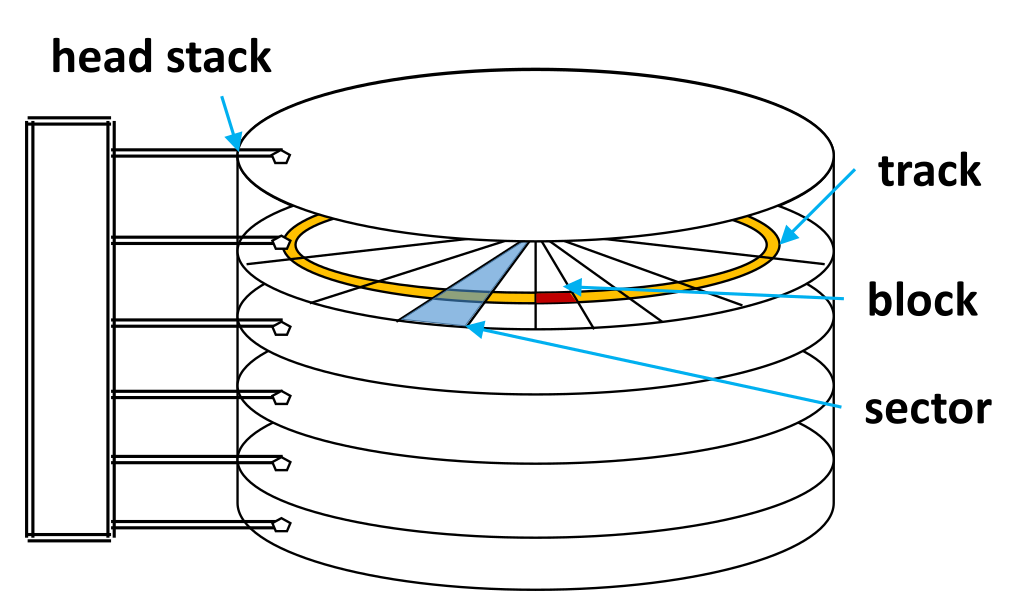
\includegraphics{hdd-structure.png}
  }
  \caption{Structure of a mechanical hard drive}
  \label{figure:hdd-structure}
  \bigskip
\end{figure}

\subparagraph*{Access Time}
The access time of the secondary memory can be measured as the sum of:
\begin{itemize}
  \item \textbf{seek} time \(8-12 \, ms\), head positioning time on the correct track
  \item \textbf{latency} time \(2-8 \, ms\), disc rotation on the correct sector
  \item \textbf{transfer} time \(0.1-1 \, ms\), data transfer from the disk to the buffer
\end{itemize}

The cost of access to secondary memory is about \(4\) orders of magnitude (\(10^4\)) higher than the one of access to main memory.
In I/O bound applications, the cost exclusively depends on the number of accesses to secondary memory.

The cost of a query is closely related to the number of numbers that are read (moved) from secondary memory.

\subparagraph*{\dbms and file systems}
The File System \textit{(FS)} is the layer of the operating system that manages the secondary memory:
\dbms make limited use of FS functionalities \textit{(such as creating or deleting files, reading or writing blocks, etc.)}, since they manage directly the file organization, both in terms of the distribution of data within the blocks and with respect to the internal structures of the blocks.
Furthermore, a \dbms may also control the physical allocation of blocks onto the disk, to optimize the access time or increase the reliability.

\subparagraph*{Data dictionary}

Each relational \dbms maintains a \textbf{data dictionary} that contains information about the database structure and the database itself.
The data dictionary is a centralized repository of information about data such as meaning, relationships to other data, origin, usage and format.

\subsection{Blocks and tuples}

The files can be split into their physical and logical components:

\begin{itemize}
  \item \textbf{blocks}: the physical components
  \item \textbf{tuples}: the logical components
\end{itemize}

While the size of a block is typically fixed, depending on the file system and on how the disk is formatted, the size of a tuple depends on the database design and is typically variable within a file.

\subparagraph*{Organization of tuples in blocks}

A block for sequential and hash-based methods is divided in:

\begin{itemize}
  \item \textbf{block header} and \textbf{trailer} with control information used by the File System
  \item \textbf{page header} and \textbf{trailer} with control information about the access method
  \item a \textbf{page dictionary} containing pointers to each elementary item of useful data contained in the page
  \item a \textbf{useful part} containing the data
        \begin{itemize}
          \item normally, page dictionaries and useful data grow as a stack in opposite directions
        \end{itemize}
  \item a \textbf{checksum} to verify the integrity of the block
\end{itemize}

An illustration of a block is shown in Figure~\ref{fig:block-structure}.

\begin{figure}[htbp]
  \centering
  \bigskip
  \tikzfig{figure-14.tikz}
  \caption{Structure of a block}
  \label{fig:block-structure}
  \bigskip
\end{figure}

\bigskip
The block factor B represents the number of tuples within a block.
It's fundamental to estimate the cost of queries:

\begin{itemize}
  \item the average \textbf{size} of a \textbf{record} \textit{(or tuple)} is called \textbf{SR}
  \item the average \textbf{size} of a \textbf{block} is called \textbf{SB}
\end{itemize}

The block factor is defined as:
\[ B = \left\lfloor \frac{\text{SB}}{\text{SR}} \right\rfloor \]
The rest of the space can be:

\begin{itemize}
  \item \textbf{used} if the records are \textbf{spanned} between block
  \item \textbf{not used}, if the records are \textbf{unspanned}
\end{itemize}

\subparagraph*{Buffer Operations}

Operations are performed in the main memory and affect the pages: in the cost model, it's always assumed that all the pages have equal size and are organized in blocks.

Operations are:

\begin{itemize}
  \item \textbf{insertion} an update of a tuple
        \begin{itemize}
          \item may require a reorganization of the page or the usage of a new page
          \item an update to a file may require a reorganization of the page
        \end{itemize}
  \item \textbf{deletion} of a tuple
        \begin{itemize}
          \item often carried out by marking the tuple as invalid and triggering later a reorganization of the page
        \end{itemize}
  \item \textbf{access} to a field of a tuple
        \begin{itemize}
          \item identified by a pointer to the beginning of the tuple and the length of the field itself
        \end{itemize}
\end{itemize}

\subsection{Indexes}

Indexes are data structures that help efficiently retrieve tuples according to certain criteria, called \textbf{search key} (or \textit{SK}); index entries are sorted with regard to the search key.

They contain records in the form \texttt{<search key pointer to block>}.

It's important to highlight the difference between \textbf{primary key} and \textbf{search key}:
the former is the key used to uniquely identify a tuple, while the latter is the key used to retrieve tuples according to certain criteria.
Furthermore, the search key defines a \textbf{search domain}: each tuple is associated with one or more pointers; each of them may not be unique.

A comparison of the two entities is shown in Table~\ref{tab:primary-key-search-key}.

\begin{table}[htbp]
  \centering
  \bigskip
  \begin{tblr}{colspec={c|c}, row{1}={font=\itshape}}
    primary key                & search key                   \\
    \hline
    does not imply access path & defines a common access path \\
    defines a constraint       & defines a common access path \\
    unique                     & not necessarily unique       \\
    implemented by an index    & -                            \\
  \end{tblr}
  \caption{Comparison between primary key and search key}
  \label{tab:primary-key-search-key}
  \bigskip
\end{table}

Indexes are smaller than primary data structures, and they can be loaded in a file in the main memory;
they support point queries, range queries, and sorted scans efficiently.
However, adding indexes to tables means that the \dbms has to update each index after an insert, update, or delete operation:
this operation may be costly and may slow it down.

\bigskip
Indexes can be categorized into \textbf{sparse} and \textbf{dense}:
while the former associate a search key to a single tuple, the latter associate a search key to a block of tuples.

\subparagraph*{Sparse indexes}
\begin{itemize}
  \item an entry index is associated with \textbf{every} search-key value in the file
  \item \textbf{high performances}: to access a tuple, the index is accessed first, and then the block is accessed
  \item can be used on \textbf{entry-sequenced} primary structures
\end{itemize}

\subparagraph*{Dense indexes}
\begin{itemize}
  \item an entry index is associated only with \textbf{some} search-key values in the file
  \item requires \textbf{less space}, but it's generally slower in locating the tuple
  \item requires\textbf{ sequentially ordered} primary structures
        \begin{itemize}[label=\(\rightarrow\)]
          \item the search key corresponds to the ordering key of the tuple
        \end{itemize}
  \item \textbf{low performances}: to access a tuple, it's necessary to scan each block until the search key is found; then the block must be scanned to locate the tuple itself
  \item good \textbf{tradeoff} between memory and performance as only one index entry is necessary for each block in the file
\end{itemize}

\subsubsection{Indexing techniques}

The index can be further classified according to the indexing used, creating the following indexes: \textbf{primary}, \textbf{secondary}, and \textbf{clustering}.

\subparagraph*{Primary index}
A primary index is defined on sequentially ordered structures.
The search key \textit{(SK)} is unique and coincides with the attribute according to which the structure is ordered:
\begin{align*}
  \text{search key} \  & = \ \text{ordering key} \\
  \text{SK} \          & = \ \text{OK}
\end{align*}

\begin{itemize}
  \item Only one primary index can be defined for each table
        \begin{itemize}
          \item usually the primary index corresponds to the primary key of the table
        \end{itemize}
  \item The index can be either \textbf{sparse} or \textbf{dense}
\end{itemize}

\subparagraph*{Secondary index}
A secondary index specifies an order different from the sequential order of the file:
\begin{align*}
  \text{search key} \  & \neq \ \text{ordering key} \\
  \text{SK} \          & \neq \ \text{OK}
\end{align*}

\begin{itemize}
  \item Multiple secondary index structures can be defined for the same table on multiple search keys
  \item It is always \textbf{dense} because tuples with contiguous values of the key can be distributed in different blocks
\end{itemize}

\subparagraph*{Clustering index}
A clustering index is a generalization of the primary index in which the ordering key \textit{(equal to the search key)} can not be unique.

\begin{itemize}
  \item The pointer of key \texttt{x} refers to the block containing the first tuple with key \texttt{x}
  \item The index can be either \textbf{sparse} or \textbf{dense}, but it is usually \textbf{sparse}
\end{itemize}

\subsubsection{Indexes in \sql}

To create an \sql index, every table should have:

\begin{itemize}
  \item a suitable \textbf{primary storage}, possibly sequentially ordered \textit{(normally on unique values)}
  \item several \textbf{secondary indexes}, both unique and non, on the attributes most used for selections and joins
        \begin{itemize}
          \item secondary structures are progressively added, checking that they are used by the system
        \end{itemize}
\end{itemize}

Guidelines for choosing indexes:

\begin{enumerate}
  \item do not index \textbf{small tables}
  \item index \textbf{primary key }of a table only if it is not a key of the primary file organization
  \item add a \textbf{secondary index} to any column that is heavily used as a \textbf{secondary key}
  \item add secondary index structures on columns that are involved in \texttt{SELECT} or \texttt{JOIN} criteria, \texttt{ORDER BY}, \texttt{GROUP BY}, and other operations involving sorting
  \item \textbf{avoid} indexing a column or table that is \textbf{frequently updated}
  \item \textbf{avoid} indexing a column if the query will retrieve a \textbf{significant number of rows}
  \item \textbf{avoid} indexing columns that consists of \textbf{long strings}
\end{enumerate}

The \sql syntax for creating and deleting an index is shown in Code~\ref{code:sql-syntax-index}.

\begin{lstlisting}[language=SQL, caption={\sql syntax for creating and deleting an index}, label={code:sql-syntax-index}]
-- creation
CREATE [UNIQUE] INDEX <index_name> on <table_name>[(<column_name>, ...)]
-- deletion
DROP INDEX <index_name>
\end{lstlisting}

\subsection{Physical Access Structures}

Each \dbms has a distinctive and limited set of access methods and software modules that provide data access and manipulation (\texttt{STORE} and \texttt{RETRIEVE}) primitives for each physical data structure.

Access methods have their own data structures to organize data:

\begin{itemize}
  \item Each table is stored in exactly \textbf{one primal} physical data structure
  \item Each table may have \textbf{zero or more secondary} access structures
\end{itemize}

\bigskip
Structures are divided in two \textbf{categories}:

\begin{itemize}
  \item \textbf{Primary}: contains  all the tuples of a table; its main purpose is store the table content
  \item \textbf{Secondary}: used to index primary structures, and only contains the values of some fields, interleaved with pointers to the block of the primary structure; its main purpose is to speed up the search for specific tuples, according to some criteria
\end{itemize}

To access each type of structure, the \dbms uses a different set of access methods:

\begin{itemize}
  \item \textbf{Sequential} access methods
  \item \textbf{Hash-based} access methods
  \item \textbf{Tree-based} access methods
\end{itemize}

Not all types of structures are equally suited for implementing the primary or secondary access methods, as shown in Table~\ref{tab:access-structures}.

\begin{table}
  \centering
  \bigskip
  \begin{tblr}{colspec={r|l|l}, row{1}={font=\itshape}, column{1}={font=\bfseries}}
               & primary                     & secondary             \\
    \hline
    sequential & \colorcmark (typical)       & \colorxmark           \\
    hash-based & \colorcmark (in some \dbms) & \colorcmark           \\
    tree-based & \colorxmark (obsolete)      & \colorcmark (typical)
  \end{tblr}
  \caption{Access structures}
  \label{tab:access-structures}
  \bigskip
\end{table}

\subsubsection{Sequential structures}
Sequential structures arrange tuples in a sequence in the secondary memory;
blocks can be contiguous on disk or sparse.

Two types of sequential structures are:

\begin{itemize}
  \item \textbf{entry-sequenced} organization: the sequence of tuples is dictated by their \textbf{entry order}
  \item \textbf{sequentially-ordered} organization: the sequence of tuples is dictated by the \textbf{value of one or more keys}
\end{itemize}

\subparagraph*{Entry-sequenced organization} Entry-sequenced organization \textit{(also called heap)} is the simplest and most common type of sequential organization.

\begin{itemize}
  \item \textbf{Efficient} for:
        \begin{itemize}[label=\cmarkthin]
          \item insertion, which does not require shifting
          \item space occupancy, as it uses all the blocks available for data and all the space within a block
          \item sequential reading and writing, especially if the blocks are contiguous
          \item query like \texttt{SELECT * FROM table}
        \end{itemize}
  \item \textbf{Inefficient} for:
        \begin{itemize}[label=\xmarkthin]
          \item searching specific data units, as it may require scanning the whole structure
                \begin{itemize}[label=\(\rightarrow\)]
                  \item this issue can be solved via indexes
                \end{itemize}
          \item updates that increase the size of a tuple, as it may require shifting and writing on another block
                \begin{itemize}[label=\(\rightarrow\)]
                  \item this issue can be solved by deleting old versions of the tuple and inserting new ones
                \end{itemize}
          \item query like \texttt{SELECT * FROM table WHERE ...}
        \end{itemize}
\end{itemize}

\subparagraph*{Sequentially-ordered sequential structure}
Tuples are sorted according to the value of a key field.

\begin{itemize}
  \item Efficient for:
        \begin{itemize}[label=\cmarkthin]
          \item range queries that retrieve tuples having the key in an interval
          \item \texttt{order by} and \texttt{group by} queries exploiting the key
        \end{itemize}
  \item Inefficient for:
        \begin{itemize}[label=\xmarkthin]
          \item reordering tuples within a block, if there is even enough space
        \end{itemize}
\end{itemize}

To avoid the global reordering problem, the following techniques can be used:

\begin{itemize}
  \item \textbf{Differential files} and periodic \textbf{merging}
  \item \textbf{Local reordering} operation within a block
  \item \textbf{Creation of an overflow file} that contains tuples that do not fit in the current block
\end{itemize}

\paragraph{Comparison of sequential structures}

Table~\ref{tab:sequential-structures} shows the main differences between the main structures.

In real-world applications, the entry-sequenced organization is the most common solution only if paired with secondary access structures.

\begin{table}[htbp]
  \centering
  \bigskip
  \begin{tblr}{colspec={r|c|c}, row{1}={font=\itshape}, cell{2-5}{1}={font=\ttfamily}, cells={valign=m}}
                                & entry-sequenced & sequentially-ordered \\
    \hline
    INSERT                      & \colorcmark     & \colorxmark          \\
    UPDATE                      & \colorcmark     & \colorxmark          \\
    DELETE                      & \colorxmark     & \colorxmark          \\
    SELECT * FROM T WHERE [...] & \colorxmark     & \colorcmark          \\
  \end{tblr}
  \caption{Comparison of sequential structures}
  \label{tab:sequential-structures}
  \bigskip
\end{table}

\subsubsection{Hash-based structures}

\textbf{Hash-based} structures provide efficient associative access to data, based on the value of a key field.

A hash-based structure has \(N_B\) buckets, with \(N_B \ll \# \ \text{of data items}\):
a bucket is a unit of storage, typically of the size of \(1\) block;
often they are stored adjacently in the file.
A hash function maps the key field to a value between \(0\) and \(N_B -1\);
this value is interpreted as the index of a bucket in the hash structure (via a hash table).

\begin{itemize}
  \item \textbf{Efficient} for:
        \begin{itemize}[label=\cmarkthin]
          \item tables with small size and almost static content
          \item queries with equality predicates on the key field \textit{(point queries)}
        \end{itemize}
  \item \textbf{Inefficient} for:
        \begin{itemize}[label=\xmarkthin]
          \item tables with large size and dynamic content
          \item queries with inequality predicates on the key field \textit{(range queries)}
        \end{itemize}
\end{itemize}

\subparagraph*{Implementation}
The implementation consists of two steps.

\begin{enumerate}[label=step \arabic*., leftmargin=*, widest*=7, labelindent=1em]
  \item \textbf{folding}: transforms the key values to positive integers, uniformly distributed in a big range
  \item \textbf{hashing}: transforms the positive number into an index in range \(\left[ 0, N_B - 1 \right]\), to be used as the index of a bucket
\end{enumerate}

\subparagraph*{Collision}
When two or more keys are mapped to the same bucket, a \textbf{collision} occurs;
when the number of tuples in a block is greater than the number of buckets, collisions are inevitable.

Techniques to solve collisions:

\begin{itemize}
  \item \textbf{Closed hashing} \textit{(open addressing)}, where the collision is resolved by probing the next bucket
        \begin{itemize}[label=\(\rightarrow\)]
          \item a simple technique is linear probing, where the following buckets are tried in sequence wrapping around the end of the hash table
        \end{itemize}
  \item \textbf{Open hashing} \textit{(separate chaining)}, where the collision is resolved by storing the tuple in a linked list
        \begin{itemize}[label=\(\rightarrow\)]
          \item a new bucket is allocated for the same hash result linked to the previous one
        \end{itemize}
\end{itemize}

\subparagraph*{Overflow chains}
The average length of the overflow chain is a function of:

\begin{itemize}[itemsep=0.5ex]
  \item the \textbf{load factor} \(\alpha = \dfrac{T}{B \times N_B}\), representing the average occupancy of a block
  \item the \textbf{block factor} \(\beta = \dfrac{B}{\# \ \text{of items}} = \dfrac{1}{\alpha}\), representing the average number of items per block
\end{itemize}

Where:

\begin{itemize}
  \item \(T\) is the \textbf{number} of \textbf{tuples}
  \item \(N_B\) is the \textbf{number} of \textbf{buckets}
  \item \(B\) is the \textbf{number} of \textbf{tuples within a block}
\end{itemize}

\paragraph{Hash-based indexes}

Hash-based structures can be used for \textbf{secondary index structures}:
they are shaped and managed exactly like a hash-based primary structure, but instead of the tuples, the buckets contain key values and pointers.

In a huge database it would be very inefficient to search all the index values to reach the desired data:
a good performance equality query predicates on the key field.
This technique is as such inefficient for access based on interval predicates or the value of non search-key attributes.

\subsubsection{Tree-based structures}

The tree-based structures are the most frequently used in relational \dbms for secondary index structures;
for instance, \sql structures are implemented this way.
They support associative access based on the value of a key search field.

A commonly used tree-based structure is the \textbf{B-tree}.

\subparagraph*{B-trees}
Balanced trees \textit{(or B-trees)} are a generalization binary search trees;
the length of all the possible paths from the root node to the leaves is the same, while a node can have any number of children in a predefined range.
This constraint improves the performance of the database.

There are two types of B-trees:

\begin{enumerate}
  \item \textbf{B trees}: the key values are stored in \textbf{leaf nodes and internal nodes}
  \item \textbf{B+ trees}: the key values are stored in \textbf{leaf nodes} only
\end{enumerate}

\paragraph{B+ trees}

The \textbf{B+ tree} represents an evolution from the B-tree.
Each node is stored in a block, and the key values are stored in the leaf nodes only;
since the majority of the nodes are leaf nodes, the B+ tree is more efficient than the B-tree.

The fan-out depends on the size of the block, the size of the key and the size of the pointer.

\subparagraph*{Structure of an internal node}
The structure of an internal node is shown in Figure~\ref{subfig:b-tree-internal-node}.
Each node contains \(F\) keys, sorted lexicographically, and \(F + 1\) pointers to the child nodes.
Each key \(K_j, \ 1 \leq j \leq F\) is followed by a pointer \(P_j\), while \(K_1\) is preceded by a pointer \(P_0\).
Each pointer addresses a sub-tree:

\begin{itemize}
  \item \(P_0\) points to the subtree containing all the keys less than \(K_1\)
  \item \(P_F\) points to the subtree containing all the keys greater or equal to \(K_F\)
  \item each intermediate pointer addresses a sub-tree that contains all the information about the keys \(K\) included in the interval \(K_j \leq K < K_{j + 1}\)
\end{itemize}

The value of \(F\) depends on the size of the page and the amount of space occupied by the key values and the pointers.

\subparagraph*{Structure of a leaf node}
The structure of a leaf node is similar to the one of an internal node, but it contains only pointers to the data tuples or the data tuples themselves;
the nodes can be structured in two ways:

\begin{enumerate}
  \item the leaf node contains the entire tuple
        \begin{itemize}
          \item the data structure is called \textbf{key-sequenced}
          \item the position of a tuple is determined by the value of its key
          \item it's simple to insert or change a tuple
        \end{itemize}
  \item the leaf node contains pointers to the blocks of the database that contain tuples with the same key value
        \begin{itemize}
          \item the data structure is called \textbf{indirect}
          \item the tuples can be anywhere in the file, allowing the access of a tuple allocated via any other primary mechanism
          \item the structure of such a leaf node is shown in Figure~\ref{subfig:b-tree-leaf-node}
        \end{itemize}
\end{enumerate}

\begin{figure}[htbp]
  \centering
  \bigskip
  \begin{subfigure}{0.99\textwidth}
    \centering
    \bigskip
    \tikzfig{figure-15.tikz}
    \caption{Internal node}
    \label{subfig:b-tree-internal-node}
    \bigskip
  \end{subfigure}
  \bigskip
  \begin{subfigure}{0.99\textwidth}
    \centering
    \bigskip
    \tikzfig{figure-16.tikz}
    \caption{Leaf node}
    \label{subfig:b-tree-leaf-node}
    \bigskip
  \end{subfigure}
  \caption{Structure of the nodes of a B+ tree}
  \label{fig:b-tree-structure}
\end{figure}

\paragraph{Search Mechanism}

The search mechanism consists of the following pointers starting from the root.
At each intermediate node:

\begin{itemize}
  \item if \(V < K_1\), follow the pointer \(P_0\)
  \item If \(V \geq K_F\), follow the pointer \(P_F\)
  \item otherwise, follow the pointer \(P_j\) such that \(K_j \leq V < K_{j + 1}\)
\end{itemize}

The search continues until a leaf node is found:

\begin{itemize}
  \item in case of a key-sequenced leaf node, the search is completed as the tuple is found
  \item in case of an indirect leaf node, it's necessary to access the memory block pointed by the pointer \(P_j, \ 0 \leq j \leq F\)
\end{itemize}

\paragraph{Difference between B and B+ trees}

In B+ trees, leaf nodes are linked by a chain of pointers, connecting them in the order imposed by the key values.
This chain allows efficient execution of range queries, as it's possible to access the lower bound of the interval via a normal search and then scan sequentially the leaves until a value greater than the upper bound is found.
This data structure makes possible an ordered scan of the entire database, which is not possible in B trees.

In B trees, there is no such chain of pointers, and the only way to access the tuples in a given range is to perform a search for each tuple.
In this case, intermediate nodes use two pointers for each value \(K_i\):
one of the two is used to point directly to the block containing the tuple corresponding to \(K_i\), thus interrupting the search;
the other one is used to continue the search in the subtree that includes the key values great than \(K_i\) and less than \(K_i + 1\).
The first pointer \(P_0\) highlights the subtree corresponding to key values less than \(K_1\), while the last pointer \(P_F\) highlights the subtree corresponding to key values greater than \(K_F\).
This technique saves space in the pages of the index and at the same time allows the termination of the search when a given key value is found on intermediate nodes, without having to continue the search in the subtrees.

\subsection{Query Optimization}

The \textbf{optimizer} is an important part of the architecture of a \dbms:
it receives a query expressed in \sql, analyses the query to find mistakes, and finally generates a program in an internal format that uses the data access methods.
There may be different ways to execute the same query, and the optimizer has to choose the best one.

Steps of this operation:

\begin{enumerate}
  \item \textbf{lexical}, \textbf{syntactic} and \textbf{semantic} \textbf{analysis} of the query
  \item translation into an \textbf{internal representation} \textit{(similar to algebraic expressions)}
  \item \textbf{algebraic} optimization
  \item c\textbf{ost-based} optimization
  \item \textbf{code} generation
\end{enumerate}

\subsubsection{Relation profiles}

Each commercial \dbms possesses quantitative information about the relations in the database, called \textbf{relation profiles}.

The profile of a relationship contains the following information:

\begin{itemize}
  \item the \textbf{cardinality} \textit{(number of tuples)} CARD\((T)\) of each \textbf{table} \(T\)
  \item the \textbf{dimension} in bytes SIZE\((T)\) of each \textbf{tuple} in table \(T\)
  \item the \textbf{dimension} in bytes SIZE\((A_j, T)\) of each \textbf{attribute} \(A_j\) in \textbf{table} \(T\)
  \item the \textbf{number} of \textbf{distinct values }VAL\((A_j, T)\) of each \textbf{attribute} \(A_j\) in \textbf{table} \(T\)
  \item the \textbf{minimum} and \textbf{maximum values} MIN\((A_j, T)\) and MAX\((A_j, T)\) of each \textbf{attribute} \(A_j\) in \textbf{table} \(T\)
\end{itemize}

The relation profiles are calculated from the data stored in the tables and updated periodically via appropriate system primitives \textit{(such as the command \texttt{UPDATE STATISTICS} in Oracle \dbms)}.

Cost-based optimization requires the knowledge of an approximate value of each of the quantities contained in the relation profiles.

\bigskip
The probability that any row will satisfy a given predicate is called the \textbf{selectivity} of the predicate.

If VAL\((A) = N\) and the values are uniformly distributed, the selectivity of the predicate \(A = v\) is \(\sfrac{1}{N}\).
If no data on distribution is available, then the distribution is always assumed uniform.

\subsubsection{Internal representation of queries}

The representation that the optimizer creates for a query must account for the physical structure used to implement the tables, as well as the indexes that may be present;
the internal representation of a query uses a tree structure, where leaves correspond to the physical data structures and whose intermediate nodes represent data access operations.

Typically, the operations that can be performed on the intermediate nodes include sequential scans, orderings, indexed accesses and joins.

\subparagraph*{Scan operation}
A scan operation performs sequential access to all the tuples of a table while executing operations of algebraic or extra algebraic nature, such as:

\begin{itemize}
  \item \textbf{projection} of a subset of the attributes
  \item \textbf{selection} of a simple predicate of type \(A_i = v\)
  \item \textbf{ordering}, insertions, deletions, and modification of the tuples when they are accessed by the scan
\end{itemize}

\subparagraph*{Indexed access operation}
As already seen, indexes are structures of the database that allow to access the tuples of a table in a more efficient way than a sequential scan;
as a consequence, if the query presents only one supported predicate, it's convenient to use the corresponding index.

When a query presents a conjunction of predicates, the \dbms chooses the most selective one for the primary access via index, while the other one is evaluated later in main memory via a sequential scan;
on the other hand, if the query presents a disjunction of predicates, the \dbms is forced to do a sequential scan if any of the predicates are not supported by an index.

\subparagraph*{Join operation}
The \texttt{JOIN} operation is considered to be the most expensive for a \dbms, as there is a risk of explosion of the number of tuples in the result;
to solve this problem, the optimizer uses one of three techniques:

\begin{enumerate}
  \item \textbf{nested-loop}, based on scanning
        \begin{itemize}
          \item a scan is performed on a table \textit{(termed external)} and for each tuple, a scan is performed on the other table \textit{(termed internal)}
          \item the matching is efficient if there is an index on the join attribute of the internal table
        \end{itemize}
  \item \textbf{merge-scan}, based on ordering
        \begin{itemize}
          \item this technique requires that both the tables are sorted on the join attribute
          \item two coordinated scans run through the tuples of each table, in parallel, and the matching is performed
        \end{itemize}
  \item \textbf{hash-join}, based on hashing
        \begin{itemize}
          \item this technique requires that both tables are hashed on the join attribute
          \item the tuples of the internal table are hashed and stored in a hash table, while the tuples of the external table are scanned and the matching is performed
        \end{itemize}
\end{enumerate}

\subparagraph*{Equality}
The cost of an equality lookup \textit{(such as \(A = v\))} depends on the type of structure representing the table.

\begin{itemize}
  \item \textbf{Sequential structures} with no index:
        \begin{itemize}[label=\xmarkthin]
          \item equality lookups are \textbf{not supported}, so the cost is the one of a full scan
          \item sequentially ordered structures may have reduced cost
        \end{itemize}
  \item \textbf{Hash or Tree structures}
        \begin{itemize}[label=\cmarkthin]
          \item equality lookups are \textbf{supported} if \(A\) is the \textbf{search key attribute} of the structure
          \item the cost depends on the storage type \textit{(primary or secondary)} and the search key type \textit{(unique or not)}
        \end{itemize}
\end{itemize}

\subparagraph*{Range}
The cost of a range lookup \textit{(such as \(v_1 \leq A \leq v_2\))} depends on the type of structure representing the table.

\begin{itemize}
  \item \textbf{Sequential structure}s \textit{(primary)}:
        \begin{itemize}[label=\xmarkthin]
          \item range lookups are \textbf{not supported}, so the cost is the one of a full scan
          \item sequentially ordered structures may have reduced cost
        \end{itemize}
  \item \textbf{Hash structures} \textit{(primary and secondary)}:
        \begin{itemize}[label=\xmarkthin]
          \item range lookups are \textbf{not supported}, so the cost is the one of a full scan
        \end{itemize}
  \item \textbf{Tree structure}s \textit{(primary and secondary)}:
        \begin{itemize}[label=\cmarkthin]
          \item range lookups are \textbf{supported} if \(A\) is the \textbf{search key attribute} of the structure
          \item the cost depends on the storage type \textit{(primary or secondary)} and the search key type \textit{(unique or not)}
        \end{itemize}
  \item B\textbf{+ tree} structures \textit{(primary and secondary)}:
        \begin{itemize}[label=\cmarkthin]
          \item range lookups are \textbf{supported} if \(A\) is the \textbf{search key attribute} of the structure
        \end{itemize}
\end{itemize}

\subparagraph*{Conjunction}
If supported by indexes, the \dbms chooses the most selective supported predicate for the data access, and the other predicates are evaluated later in the main memory via a sequential scan.

\subparagraph*{Disjunction}
If any of the predicates are not supported by indexes, then a sequential scan is performed;
otherwise, indexes can be used to evaluate all predicates and then the results are merged and duplicates are removed.

\subparagraph*{Sort}
Various methods allow sorting the tuples of a table optimally;
however, the problem lies in the fact that the \dbms must load the entire loaded data in the buffer, which may be too large for the available memory.

Data can be sorted in the main memory \textit{(in which case it's performed via ad-hoc algorithms such as quicksort or merge sort)} or in the disk \textit{(in which case it's performed via external sorting algorithms)}.
The latter case is picked when the data is too big to fit on the main memory; the procedure is as follows:

\begin{enumerate}
  \item split the data in chunks of size equal to the main memory
        \item\label{enum:merge-sort-2} load a chunk in the main memory
  \item sort the data in the main memory
  \item store the sorted data back on disk
  \item Merged sorted chunks parts using at least three pages:
        \begin{itemize}
          \item two for progressively loading data from two sorted chunks
          \item one as output buffer to store the sorted data
        \end{itemize}
  \item save the result on disk
  \item go to step \ref{enum:merge-sort-2} until all chunks are merged
\end{enumerate}

\subsubsection{Cost-based Optimization}

Cost-based optimization is an optimization problem whose decisions are:

\begin{itemize}
  \item \textbf{which data} access operations to perform
  \item \textbf{in which order} to perform the operations
  \item if there are multiple options for a given operation, \textbf{which one }to choose
  \item if the query requires sorting, \textbf{how to sort} the data
\end{itemize}

In order to solve the problem, the \dbms makes use of data profiles and approximate cost formulas.
A decision tree is built, in which:

\begin{itemize}
  \item each \textbf{internal node} represents a \textbf{decision point} \textit{(a choice between two or more options)}
  \item each \textbf{leaf node} represents a \textbf{specific plan} \textit{(a sequence of operations)}
\end{itemize}

By assigning a cost to each plan, it's possible to find the optimal one via techniques of operations research such as branch and bound.
Optimizers should be able to handle these kinds of problems in a short enough time.

\subsubsection{Approaches to Query Evaluation}

The query is evaluated by the \dbms according to two techniques:

\begin{enumerate}
  \item \textbf{compile and store}
        \begin{itemize}
          \item the query is compiled and stored in the \dbms to be executed later
          \item the internal code is stored in the \dbms together with an indication of the dependencies of the code on the particular versions of the catalogue used at compile time
          \item On relevant changes in the catalogue, the compilation of the query is invalidated and the query is recompiled
        \end{itemize}
  \item \textbf{compile and go}
        \begin{itemize}
          \item the query is compiled and executed immediately, without storing the compiled code
          \item although not stored, the code may live for a while in the \dbms to be reused by other executions
        \end{itemize}
\end{enumerate}

\clearpage

\section{Ranking}

The objective of \textbf{ranking} is to find the best possible result for a given query.
It is formulated as a multi-objective optimization problem, in which the objective is the simultaneous optimization of multiple criteria \textit{(such as different attributes of objects in a dataset)}.
A general formulation is:

\begin{center}
  Given \(N\) \textbf{objects} described by \(d\) \textbf{attributes} and a notion of \textbf{goodness} \(g_i\) for each object \(i\),\\ find the \(k\) objects that maximize the goodness.
\end{center}

The two main approaches are:

\begin{enumerate}
  \item \textbf{Ranking} \textit{(or top-k)} Queries, in which the objective is to find the \(k\) objects that maximize \(g_i\)
  \item \textbf{Skyline} Queries, in which the objective is to find the objects that maximize \(g_i\) and are not dominated by any other object
\end{enumerate}

\subsection{Rank Aggregation}

The rank Aggregation problem regards finding the best possible entity among a set of \(n\) candidates based on the ranking of \(m\) voters.
Once more, two different approaches are possible:

\begin{enumerate}
  \item \textbf{Borda's} proposal: the entity with the lowest sum of ranks is the best one
  \item \textbf{Cordocet's} proposal: a candidate who defeats every other candidate in a pairwise comparison is the best one
        \begin{itemize}[label=\xmarkthin]
          \item if preferences graph contains a cycle, the winner may not exist
        \end{itemize}
\end{enumerate}

\bigskip
Since a unique solution does not exist nor does a unique way to find it, the problem is formulated as a multi-objective optimization problem;
different approaches have been defined to solve it.

\subparagraph*{Axiomatic Approach}
Arrow stated a list of \(5\) axioms that a solution to the problem must satisfy:

\begin{enumerate}[label=axiom \arabic*., leftmargin=*, labelindent=1em, widest*=8]
  \item \textbf{Non-dictatorship}: the winner cannot be chosen by a single voter
  \item \textbf{Universality}: the winner should represent the opinion of all voters
  \item \textbf{Transitivity}: if candidate \(x\) is preferred over candidate \(y\) and candidate \(y\) is preferred over candidate \(z\), then candidate \(x\) should be preferred over candidate \(z\)
  \item \textbf{Pareto-efficiency}: for every pair \(\left( x, y \right)\) of alternatives, if \(x\) is preferred over \(y\) by every voter, then \(x\) should be preferred over \(y\) by the winner
  \item \textbf{Independence of irrelevant alternatives}: if candidate \(x\) is preferred over candidate \(y\) by every voter, then the winner should be indifferent between \(x\) and \(y\)
\end{enumerate}

He then promptly proved the \textbf{Arrow's Impossibility Theorem}: when more than \(2\) or alternatives are present, no solution satisfies all the axioms;
the axioms are then inconsistent with each other and as such, they stop being axioms.

\subparagraph*{Metric Approach}
The metric approach is based on the idea of defining a finding a new ranking \(R\) whose total distance from the original rankings \(R_1, \, \ldots \, R_n\) is minimized.
Multiple distances have been defined, such as:
\begin{itemize}
  \item \textbf{Kendall Tau distance} \(K\left( R_1, R_2 \right)\), defined as the number of exchanges needed in a bubble sort algorithm to convert \(R_1\) into \(R_2\)
        \begin{itemize}[label=\xmarkthin]
          \item finding a solution is computationally hard \textit{(NP-complete)}
        \end{itemize}
  \item \textbf{Spearman's Footrule distance} \(F\left( R_1, R_2 \right)\) which adds up the distance between the ranks of the same items in the two rankings
        \begin{itemize}[label=\cmarkthin]
          \item finding a solution is computationally easy \textit{(polynomial)}
        \end{itemize}
\end{itemize}

These two distances are however related, since:
\[ K(R_1, R_2) \leq F(R_1, R_2) \leq 2 K(R_1, R_2) \]
Furthermore, Spearman's Footrule distance admits efficient approximations, such as the median ranking.

\subsection{Combining opaque rankings - MedRank}

Opaque rankings are defined as rankings that have no visible score;
as such, they cannot be compared directly.
To handle this problem, techniques using only the position of a candidate in the ranking have been created: one of the most famous is the MedRank method.
As an output, it provides an approximation of the Footrule distance, which is then used to find the best candidate.

\begin{itemize}
  \item[\(\leftarrow\)] \textbf{Input}: integer \(k\), ranked lists \(R_1 \,\ldots \, R_N\) of \(N\) elements
  \item[\(\rightarrow\)] \textbf{Output}: the top \(k\) elements
  \item \textbf{Procedure}:
        \begin{enumerate}[label=step \arabic*., ref=step (\arabic*), widest*=7, leftmargin=*, labelindent=1em]
          \item used sorted accesses in each list, one element at a time, until there are \(k\) elements that occur in more than \(\sfrac{m}{2}\) lists
          \item for each element that occurs in more than \(\sfrac{m}{2}\) lists, compute the median of the positions in which it occurs
          \item return the top \(k\) elements with the lowest median
        \end{enumerate}
\end{itemize}

The maximum number of sorted accesses made on each list is also called the \textbf{depth} reached by the algorithm.
When the median ranks are all distinct, the algorithm provides the best possible approximation of the Footrule distance.

\subsubsection{Instance Optimality}

\textbf{Instance Optimality} is a form of optimality applied when standard optimality is unachievable.

Let \(A\) be a family of algorithms, \(I\) a family of instances, and \(c\) a cost function that maps an algorithm and an instance to a cost.
Then algorithm \(A^\ast\) is instance optimal with regards to \(A\) and \(I\) for the cost metric \(c\) if there exists constants \(k_1, \ k_2\) such that, for all \(A_i \in A\) and \(I_j \in I\):
\[ c\left( A_i, I_j \right) \leq k_1 \cdot c\left( A^\ast, I_j \right) \leq k_2 \cdot c\left( A_i, I_j \right) \]
If \(A^\ast\) is instance-optimal, then any algorithm can improve with respect to \(A^\ast\) by only a constant factor, called the \textbf{optimality ratio} of \(A^\ast\).

Instance optimality is a much stronger notion than standard optimality in the average or worst case since it guarantees that the algorithm is optimal on every input instance.

\paragraph{Optimality of MedRank}

An algorithm is defined \textbf{optimal} if its execution cost is never worse than any other algorithm on any input.

MedRank is \textbf{not optima}l;
however, it's \textbf{instance optimal}:
among the algorithms that access the lists in sorted order, this is the best possible one \textit{(up to a constant factor)} on every input instance.

\subsection{Ranking Queries - Top-k}

The Ranking Queries technique, also called Top-k, aims to retrieve the best \(k\) answers from a (potentially large) set of \(n\) answers;
the notion of best depends on the context and application.

The method requires being able to order objects according to their relevance.

\subparagraph*{Naive approach}
Assume that \(S\) is a scoring function that assigns to each tuple \(t\) a numerical score \(S(t)\).

\begin{itemize}
  \item[\(\leftarrow\)] \textbf{Input}: cardinality \(k\), dataset \(R\) composed by a set of tuples \(t\), scoring function \(S\)
  \item[\(\rightarrow\)] \textbf{Output}: the top \(k\) tuples in \(R\) according to \(S\)
  \item \textbf{Procedure}:
        \begin{enumerate}[label=step \arabic*., ref=step (\arabic*), widest*=7, leftmargin=*, labelindent=1em]
          \item for all tuples \(t\) in \(R\), compute \(S(t)\)
          \item sort tuples according to their score
          \item return the first \(k\) highest-scoring tuples
        \end{enumerate}
\end{itemize}

This approach is expensive for large datasets, as it requires sorting a large amount of data;
furthermore, if the scoring function evaluates more than one relation, the sorting must be performed on the Cartesian product of the relations \textit{(which is even more expensive)}.

\subparagraph*{Top-k in \sql}
To perform a Top-k query in \sql, the \dbms must be capable of:

\begin{enumerate}
  \item \textbf{ordering} tuples according to a scoring function
        \begin{itemize}
          \item performed via the \texttt{ORDER BY} clause
        \end{itemize}
  \item \textbf{limiting} the output to the first \(k\) tuples
        \begin{itemize}
          \item limiting was not native in \sql until 2008
          \item performed via \texttt{FETCH FIRST k ROWS ONLY}, while many non standard syntax are available
        \end{itemize}
\end{enumerate}

Only the first \(k\) tuples become part of the result;
if more than one set of \(k\) tuples satisfies the \texttt{ORDER BY} directive, then any of such sets is a valid answer and the \dbms is free to choose one: the semantic is \textbf{non-deterministic}.

\subsubsection{Evaluation of Top-k Queries}

\paragraph{Single relation}

In the simplest case, the Top-k query is evaluated via a single relation:
\begin{itemize}
  \item if the tuples are sorted according to the scoring function, the query can be evaluated in \(O(k)\) time
        \begin{itemize}
          \item only the first \(k\) tuples are read and returned
          \item there's no need to scan the entire input
        \end{itemize}
  \item if the tuples are not sorted and \(k\) is not too large, the query can be evaluated in \(O(n\log(n))\) time
        \begin{itemize}
          \item the entire input is scanned and sorted
        \end{itemize}
\end{itemize}

\paragraph{Multiple relations}

The Top-k query can be evaluated on multiple relations: if the relations are \(2\), the attribute space can be visualized as a \(2D\) plane, where each tuple is represented by a point with coordinates \(\left( A_1, A_2 \right)\).
A representation of the Top-k query on two relations is shown in Figure \ref{fig:topk-2d-plane}.

\begin{figure}[htbp]
  \centering
  \bigskip
  \tikzfig[1.5]{figure-17.tikz}
  \caption{Top-k query on two relations}
  \label{fig:topk-2d-plane}
  \bigskip
\end{figure}

If \(S\) has form \(S = k_1 \cdot A_1 + k_2 \cdot A_2\) and the objective is minimizing it, the target value lies in \(q = \left( 0, 0 \right)\).
By fixing a value of \(S\), it's possible to calculate a slope; all the points that lie on the line are equally good answers.
A representation of the weights of the Top-k query is shown in Figure \ref{subfig:topk-weights}.

On the other hand, if the objective is getting the tuples that best match the target value \(q\), the \(k\) best tuples are the ones that are closest to \(q\): the distance between two tuples can be calculated in different ways.
A representation of the weights of the Top-k query is shown in Figure \ref{subfig:topk-target}.

\begin{figure}[htbp]
  \centering
  \bigskip
  \begin{subfigure}[t]{0.495\textwidth}
    \centering
    \bigskip
    \tikzfig[1]{figure-18.tikz}
    \caption{Top-k query weights}
    \label{subfig:topk-weights}
    \bigskip
  \end{subfigure}
  \begin{subfigure}[t]{0.495\textwidth}
    \centering
    \bigskip
    \tikzfig[1]{figure-19.tikz}
    \caption{Top-k query target}
    \label{subfig:topk-target}
    \bigskip
  \end{subfigure}
  \bigskip
\end{figure}

For this reason, it is sometimes useful to consider distances rather than scores;
therefore, the model is now a \(m\)-dimensional space of ranking attributes \(A = \left( A_1, A_2, \,\ldots\, A_m \right)\).
A relation \(R = \left( A_1, A_2, \,\ldots\, A_m, B_1, B_2 \,\ldots\, B_n \right)\) is a set of attributes, where \(A_i, \ 1 \leq i \leq m\) are the attributes of the first tuple and \(B_j, \ 1 \leq j \leq m\) are the attributes of the second tuple.
The target tuple is \(q = \left( q_1, q_2, \,\ldots\, q_m \right),\ q \in A\), while a function \(d: A \times A \rightarrow \mathbb{R}\) is used to calculate the distance between two tuples in \(A\).

\bigskip
Under this model, a Top-k query is transformed into a k-Nearest Neighbours \textit{(k-NN)} query.

\begin{itemize}
  \item[\(\leftarrow\)] \textbf{Input}: point \(q\), relation \(R\), integer \(k \geq 1\), and a distance function \(d\)
  \item[\(\rightarrow\)] \textbf{Output}: the \(k\) tuples in \(R\) that are closest to \(q\) according to \(d\)
\end{itemize}

\subsubsection{Distance Functions}

The most common class of distance functions is the \textbf{LP-norm} \textit{(or Minkowski distance)}, defined as:
\[ L_p(t, q) = \left( \displaystyle\sum_{i=1}^m \left| t_i - q_i \right|^p  \right)^{\sfrac{1}{p}} \]

Some relevant cases:

\begin{itemize}[itemsep=1ex]
  \item \(p = 1 \rightarrow L_1(t, q) = \displaystyle\sum_{i=1}^m \left| t_i - q_i \right|\), \textbf{Manhattan} distance
  \item \(p = 2 \rightarrow L_2(t, q) = \sqrt{\displaystyle\sum_{i=1}^m \left( t_i - q_i \right)^2}\), \textbf{Euclidean} distance
  \item \(p = \infty \rightarrow L_\infty(t, q) =\displaystyle \max_{i=1}^m \left| t_i - q_i \right|\), \textbf{Chebyshev} distance
\end{itemize}

The different functions generate different shapes of the attribute space:

\begin{itemize}
  \item Manhattan distance: the attribute space is a \textbf{hypercube}
  \item Euclidean distance: the attribute space is a \textbf{hypersphere}
  \item Chebyshev distance: the attribute space is a \textbf{hyper square}
\end{itemize}

\paragraph*{Distance Functions with weights}

The use of weights \(W = \left( w_1, \,\ldots\,, w_m \right)\) allows to give more importance to some attributes than others;
as a consequence, the distance function is modified and the attribute space is modified as follows:

\begin{itemize}[itemsep=1.5ex]
  \item \textbf{Manhattan} distance: \(L_1(t, q, W) = \displaystyle\sum_{i=1}^m w_i \left| t_i - q_i \right|\), the relative space is a \textbf{hyper rhomboid}
  \item \textbf{Euclidean} distance: \(L_2(t, q, W) = \sqrt{\displaystyle\sum_{i=1}^m w_i \left( t_i - q_i \right)^2}\), the relative space is a \textbf{hyper ellipsoid}
  \item \textbf{Chebyshev} distance: \(L_\infty(t, q, W) = \max_{i=1}^m w_i \left| t_i - q_i \right|\), the relative space is a \textbf{hyper rectangle}
\end{itemize}

The elongation of the attribute space is proportional to the ratio of the weights.

\subsubsection{Top-k Query in \sql}

In a Top-k query, there are \(n > 1\) input relations and a scoring function \(S\) defined on the result of the join, as shown in Code~\ref{lst:topk-query-sql}.

\begin{lstlisting}[language=sql, morekeywords={FETCH}, caption={Top-k query in \sql}, label={lst:topk-query-sql}]
SELECT <attributes>
FROM <relation 1> R1, <relation 2> R2, ..., <relation n> Rn
WHERE <join and local condition>
ORDER BY <scoring function> DESC
FETCH FIRST k ROWS ONLY
\end{lstlisting}

where the scoring function has the form \(S(p_1, p_2, \,\ldots\,, p_n)\), and \(p_i\) is the weight relative to attribute \(A_i\).

Each object \(o\) returned by the input \(L_j\) has an associated partial \textit{(or local)} score \(p_j(o) \in \left[ 0, 1 \right]\);
for convenience, the scores are normalized in the range \([0, 1]\), as only the worst and best possible scores of the objects are relevant.

\begin{itemize}
  \item The \textbf{hypercube} \(\left[ 0, 1 \right]^m\) is called the \textbf{score space}
  \item The \textbf{tuple} \(p(o) = \left( p_1(0), p_2(0), \,\ldots\,, p_m(0) \right) \in \left[ 0, 1 \right]^m\) is called the \textbf{map of \(o\) into the score space} \textit{(or score vector)}
  \item The\textbf{ global score} \(S(o)\) of \(o\) is computed via a \textbf{scoring function} \(S\) that combines the local scores of \(o\):
        \[ S: \left[ 0, 1 \right]^m \rightarrow R \ S(o) = S\left( p(o) \right) = S\left( p_1(o), p_2(o), \,\ldots\,, p_m(o) \right) \]
\end{itemize}

\paragraph{Common sorting algorithms}

The following \sql functions are commonly used to compute the global score \(S(o)\):

\begin{itemize}
  \item \texttt{SUM} (or \texttt{AVG}): weights the preferences \textbf{equally}
        \[ \texttt{SUM}(o) = \texttt{SUM}\left( p(o) \right) = \displaystyle\sum_{i=1}^m p_i(o) \]
        \[ \texttt{AVG}(o) = \texttt{AVG}\left( p(o) \right) = \frac{1}{m} \displaystyle\sum_{i=1}^m p_i(o) \]
  \item \texttt{WSUM}: weights the ranking attributes \textbf{differently}
        \[ \texttt{WSUM}(o) = \texttt{WSUM}\left( p(o) \right) = \displaystyle\sum_{i=1}^m w_i p_i(o) \]
  \item \texttt{MIN}: considers the \textbf{worst} partial score
        \[ \texttt{MIN}(o) = \texttt{MIN}\left( p(o) \right) = \min_{i=1}^m p_i(o) \]
  \item \texttt{MAX}: considers the \textbf{best} partial score
        \[ \texttt{MAX}(o) = \texttt{MAX}\left( p(o) \right) = \max_{i=1}^m p_i(o) \]
\end{itemize}

The objective is still finding the \(k\) objective with the highest global score.

\paragraph{Top-k 1-1 \texttt{JOIN} query}

The Top-k 1-1 \texttt{JOIN} query is a special case of the Top-k query, where the \texttt{JOIN} operation is a 1-1 \texttt{JOIN}:
all the joins are on common attributes.
It's the simplest case of the Top-k query.

Assumptions that allow the use of the \sql Top-k 1-1 \texttt{JOIN} query:

\begin{itemize}
  \item each input list supports \textbf{sorted access}: each access returns the id of the next best object and its partial score \(p_j\)
  \item each input list supports \textbf{random access}: each access returns the partial score of an object, given its id
  \item the \textbf{id} of an object is the \textbf{same} across all inputs
  \item each input consists of the \textbf{same set} of objects
\end{itemize}

\paragraph{Scoring Functions Model}

Two different scenarios are possible:

\begin{enumerate}
  \item an \textbf{index} is available on the \textbf{common attribute}
  \item the \textbf{relation} is spread over \textbf{several sites}, each providing information only on a subset of the tuples \textit{(middleware scenario)}
\end{enumerate}

\subparagraph*{Efficient computation of \texttt{MAX} Top-k 1-1 join query}
When the scoring function is \texttt{MAX}, the Top-k query can be calculated efficiently via the \(B_0\) algorithm.

\begin{itemize}
  \item[\(\leftarrow\)] \textbf{Input}: integer \(k \geq 1\), ranked lists \(R_1, \,\ldots\, R_m\)
  \item[\(\rightarrow\)] \textbf{Output}: the \(k\) best objects according to the \texttt{MAX} scoring function
  \item \textbf{Procedure}:
        \begin{enumerate}[label=step \arabic*., ref=step (\arabic*), widest*=7, leftmargin=*, labelindent=1em]
          \item Make \(k\) sorted access on each list and store objects and partial scores in a buffer \(B\)
          \item For each object in \(B\), compute the \texttt{MAX} of its available partial scores
          \item Return the \(k\) objects with the highest \texttt{MAX} score
        \end{enumerate}
\end{itemize}

The algorithm does not need to obtain missing partial scores and does not need random access to the lists.
Furthermore, \(B_0\) is \textbf{instance-optimal}.

\paragraph{Fagin's Algorithm}
\textbf{Fagin's algorithm} \textit{(or FA)} is described as follows.

\begin{itemize}
  \item[\(\leftarrow\)] \textbf{Input}: integer \(k \geq 1\), function \(S\) combining ranked lists \(R_1, \,\ldots\, R_m\)
  \item[\(\rightarrow\)] \textbf{Output}: the top \(k\) \texttt{<object, score>} pairs
  \item \textbf{Procedure}:
        \begin{enumerate}[label=step \arabic*., ref=step (\arabic*), widest*=7, leftmargin=*, labelindent=1em]
          \item Extract the same number of objects via sorted accesses in each list until there are at least \(k\) objects in common
          \item For each extracted object, compute its score by making random accesses to the lists
          \item Among these, return the \(k\) objects with the highest score
        \end{enumerate}
\end{itemize}

The time complexity is sub-linear in the number of objects in the lists, as it's proportional to the square root of \(N\) when combining two lists: \(\mathcal{O}\left( N^{\sfrac{m-1}{m}} k^{\sfrac{1}{m}} \right)\).
The stopping criterion is independent of the scoring function and the algorithm is not instance-optimal.

A visual representation of the algorithm is shown in Figure~\ref{fig:fagin-algorithm}:

\begin{itemize}
  \item the threshold point \(\tau\) is the point with the smallest seen values on all lists in the sorted access phase
  \item the yellow region contains the points seen in all regions
  \item the grey regions contain the points seen in at least one ranking
  \item the blue region contains the points not seen in any ranking
  \item the algorithm stops when the yellow region contains at least \(k\) points
\end{itemize}

\begin{figure}[htbp]
  \centering
  \bigskip
  \tikzfig[1.5]{figure-20.tikz}
  \caption{Visualization of Fagin's algorithm}
  \label{fig:fagin-algorithm}
  \bigskip
\end{figure}

\subparagraph*{Limits of the Fagin's Algorithm}
The limits of Fagin's algorithm are:

\begin{itemize}
  \item Specific scoring functions are not exploited at all: the costs of the random and sorted accesses are not taken into account in the scoring function
  \item Memory requirements can become prohibitive: FA has to buffer all of the objects seen in the sorted access phase
  \item Small improvements are possible only by changing the algorithm itself
  \item Significant improvements require changing the stopping condition
\end{itemize}

\paragraph{Treshold Algorithm}

The \textbf{Threshold Algorithm} \textit{(or TA)} is a variant of Fagin's algorithm that exploits the scoring function to improve the performance.

\begin{itemize}
  \item[\(\leftarrow\)] \textbf{Input}: integer \(k \geq 1\), monotone function \(S\) combining ranked lists \(R_1, \,\ldots\, R_m\)
  \item[\(\rightarrow\)] \textbf{Output}: the top \(k\) \texttt{<object, score>} pairs
  \item \textbf{Procedure}:
        \begin{enumerate}[label=step \arabic*., ref=step (\arabic*), widest*=7, leftmargin=*, labelindent=1em]
          \item\label{enum:threshold-algorithm-1} Do a sorted access in parallel in each list \(R_i\)
          \item For each object \(o\), do random accesses in the other lists \(R_j\), thus obtaining the score \(s_j\)
          \item Compute the overall score \(S\left( s_1, \,\ldots\, s_m \right)\); if the value is among the \(k\) highest, store \(o\)
          \item Let \(s_{li}\) be the minimum score (the last seen under sorted access) of ranked list \(R_i\)
          \item Define the threshold \(T = S\left( s_{l1}, \,\ldots\, s_{lm} \right)\)
          \item If the score of the \(k\)-th object is less than \(T\), go back to~\ref{enum:threshold-algorithm-1}
          \item Return the current \(k\) objects with the highest score
        \end{enumerate}
\end{itemize}

The Threshold Algorithm is instance optimal among all algorithms that use random and sorted accesses:
the stopping criterion depends on the scoring function.

A visual representation of the algorithm is shown in Figure~\ref{fig:treshold-algorithm}:

\begin{itemize}
  \item the threshold point \(\tau\) is the point with the smallest seen values on all lists in the sorted access phase
  \item the dashed red line separates the region of points with a higher score than \(\tau\) from the rest
  \item the yellow region contains the points seen in all regions
  \item the blue region contains the points not seen in any ranking
  \item the algorithm stops when the yellow region contains at least \(k\) points with a score higher than \(\tau\)
\end{itemize}

\begin{figure}[htbp]
  \centering
  \bigskip
  \tikzfig[1.5]{figure-21.tikz}
  \caption{Visualization of the Threshold algorithm}
  \label{fig:treshold-algorithm}
  \bigskip
\end{figure}

Generally speaking, the Threshold algorithm is more efficient than Fagin's algorithm, since it can adapt to the specific scoring function.
To characterize the performance of the Threshold Algorithm, it's necessary to first define the \textbf{middleware cost}:
\[ \text{cost} = S_A \cdot c_{S_A} + S_R \cdot c_{S_R} \]
where:
\begin{itemize}
  \item \(S_A\) is the number of sorted accesses
  \item \(S_R\) is the number of random accesses
  \item \(c_{S_A}\) is the cost of a sorted access
  \item \(c_{S_R}\) is the cost of a random access
\end{itemize}

In an ideal scenario, \(c_{S_A} = c_{S_R} = 1\), thus the cost is equal to the number of accesses;
in other cases, the base cost may differ:

\begin{itemize}
  \item for web sources, usually \(c_{R_A} \gg c_{S_R}\)
        \begin{itemize}
          \item limit case: \(c_{R_A} = \infty\), the random access is impossible
        \end{itemize}
  \item some sources might not be accessible through sorted access
        \begin{itemize}
          \item happens when there's no index to process an attribute \(p_j\)
          \item \(c_{S_A} = \infty\)
        \end{itemize}
\end{itemize}

\paragraph{No Random Access Algorithm}
The \textbf{No Random Access Algorithm} \textit{(or NORA)} is a variant of the Threshold Algorithm that does not use random accesses;
it still returns the Top-k results, but the scores might be uncertain.

The main idea of the algorithm is to maintain a lower bound \(S^-(o)\) and an upper bound \(S^+(o)\) of the score for each retrieved object \(o\);
to achieve such an objective, a buffer \(B\) with unlimited capacity is used and it's kept sorted according to decreasing lower bounds \(S^-(o)\).
The algorithm terminates when no new object \(\overline{o}\) can do better than any of the objects in the set.

\begin{itemize}
  \item[\(\leftarrow\)] \textbf{Input}: integer \(k \geq 1\), monotone function \(S\) combining ranked lists \(R_1, \,\ldots\, R_m\)
  \item[\(\rightarrow\)] \textbf{Output}: the top \(k\) objects according to \(S\)
  \item \textbf{Procedure}:
        \begin{enumerate}[label=step \arabic*., ref=step (\arabic*), widest*=7, leftmargin=*, labelindent=1em]
          \item\label{enum:nra-algorithm-1} Do a sorted access in parallel in each list \(R_i\)
          \item Store in \(B\) each retrieved object \(o\) and maintain \(S^-(o)\) and \(S^+(o)\) for each \(o\) and a threshold \(\tau\)
          \item Go to~\ref{enum:nra-algorithm-1} as long as there's a new object \(\overline{o}\) such that \(S^+(o) > \tau\)
        \end{enumerate}
\end{itemize}

The \textit{NRA} Algorithm is instance optimal among all algorithms that use only sorted accesses \textit{(don't use random accesses)};
the optimality ratio is \(m\).
The cost of the algorithm does not grow monotonically with \(k\):
it might be cheaper to look for the top \(k\) objects than for the top \(k - 1\) objects.

\paragraph{Comparison of the Algorithms}

Table~\ref{tab:comparison-algorithms} shows a comparison between the three algorithms.

\begin{table}[htbp]
  \centering
  \bigskip
  \begin{tblr}{colspec={c|c|c|c}, row{1}={font=\itshape}, cell{2-5}{1}={font=\ttfamily}}
    algorithm & scoring function & data access       & notes                                  \\
    \hline
    B0        & \texttt{MAX}     & sorted            & instance-optimal                       \\
    FA        & monotone         & sorted and random & cost not dependent on scoring function \\
    TA        & monotone         & sorted and random & instance-optimal                       \\
    NRA       & monotone         & sorted            & instance-optimal, no exact scores      \\
  \end{tblr}
  \caption{Comparison of the algorithms}
  \label{tab:comparison-algorithms}
  \bigskip
\end{table}

\subsection{Skyline Queries}

The Skylines Queries technique aims to retrieve the best objects in a set according to several different criteria.
Instead of specifying a score function \textit{(as in the Top-k Queries)}, the algorithm is based on the notion of \textbf{dominance}.

Tuple \(t\) \textbf{dominates} tuple \(s\) \textit{(denoted \(t \prec s\))} if and only if two conditions are satisfied:

\begin{enumerate}
  \item \(\forall \, i \ 1 \leq i \leq m: t[A_i] \leq s[A_i]\) - tuple \(t\) is better than \(s\) on all attributes
  \item \(\exists \, k \, \mid t[A_k] < s[A_j]\) - tuple \(t\) is better than \(s\) on at least one attribute
\end{enumerate}

Note that these conditions assume that a lower score is better;
the same principle applies if the objective is to maximize the score function.
This convention is the opposite of the one used in the Top-k Queries.

The \textbf{skyline} of a relation is the set of its non-dominated tuples:

\begin{itemize}
  \item Maximal vectors problem \textit{(in computational geometry)} - find the set of non-dominated points in a set of points
  \item Pareto-optimal solutions \textit{(in multi-objective optimization)} - find the set of non-dominated solutions in a set of solutions
\end{itemize}

In \(2D\), the shape of the contour of the dataset resembles a skyline \textit{(Figure~\ref{fig:skyline-2d})}.

\begin{figure}[htbp]
  \centering
  \bigskip
  \tikzfig[1.25]{figure-22.tikz}
  \caption{Skyline in 2D}
  \label{fig:skyline-2d}
  \bigskip
\end{figure}

\subparagraph*{Properties of the skyline}

\begin{itemize}
  \item A tuple \(t\) is in the skyline if and only if is the Top-1 tuple according to at least one monotone scoring function
  \item The skyline is not the Top-k query, since no scoring function yields in the first \(k\) positions the skyline points on all possible instances
\end{itemize}

\subparagraph*{Main aspects of skyline queries}

\begin{itemize}
  \item \textbf{Pros}:
        \begin{itemize}[label=\cmarkthin]
          \item \textbf{Effective} in identifying potentially interesting objects if nothing is known about the preference of a user
          \item Very \textbf{simple} to use, as no parameter is needed
        \end{itemize}
  \item \textbf{Cons}:
        \begin{itemize}[label=\xmarkthin]
          \item \textbf{Too many objects} might be returned in large, non-correlated datasets
          \item Computation is \textbf{quadratic} in the size of the dataset \textit{(and thus infeasible for large datasets)}
          \item \textbf{Agnostic} to the user's preferences
        \end{itemize}
  \item \textbf{Extension}:
        \begin{itemize}
          \item \textbf{k-skyband}: the set of tuples dominated by less than \(k\) tuples
        \end{itemize}
\end{itemize}

\subsubsection{Skyline Queries in \sql}

There's no standard \sql syntax for skyline queries;
a proposed syntax is shown in Code~\ref{code:skyline-query-proposed}.
A naively implemented skyline query would be very inefficient since it would require a full scan of the table;
an example of such an implementation is shown in Code~\ref{code:skyline-query-naive}.

\begin{lstlisting}[language=sql, morekeywords={SKYLINE}, caption={Proposed syntax for skyline queries}, label=code:skyline-query-proposed]
SELECT <attributes>
FROM <table>
GROUP BY <grouping attributes>
HAVING <condition>
SKYLINE OF [ALL | DISTINCT] <attribute> [MIN | MAX | DIFF]
  {, <attribute> [MIN | MAX | DIFF], ...}
ORDER BY <attribute> [ASC | DESC] {, <attribute> [ASC | DESC], ...}
\end{lstlisting}

\begin{lstlisting}[language=sql, caption={Naive implementation of skyline queries}, label=code:skyline-query-naive]
SELECT * FROM hotels AS h
WHERE h.city = 'Paris' AND NOT EXISTS (
  SELECT * FROM hotels AS h2
  WHERE h2.city = h1.city AND
    h1.distance <= h2.distance AND
    h1.price <= h2.price AND
    (
      h1.distance < h2.distance OR
      h1.price < h2.price
    )
)
\end{lstlisting}

\paragraph{Block Nested Loops Algorithm}

The Block Nested Loops \textit{(BNL)} Algorithm is a skyline query algorithm that uses a \textbf{block} of tuples to perform the skyline computation.

\begin{itemize}
  \item[\(\leftarrow\)] \textbf{Input}: dataset \(D\) of multi dimensional points
  \item[\(\rightarrow\)] \textbf{Output}: skyline of \(D\)
  \item \textbf{Procedure}: shown in Code~\ref{code:block-nested-loops-algorithm}
\end{itemize}

\begin{lstlisting}[caption={Block Nested Loops algorithm}, label=code:block-nested-loops-algorithm]
W := $\emptyset$
for every point p $\in$ D
  if p is not dominated by any point $in$ W
    W := W $\setminus$ {points dominated by p}
    W := W $\cup$ {p}
  end
end
\end{lstlisting}

The computation of the skyline is \(\mathcal{O}\left( n^2 \right)\), with \(n = |D|\); as such, it's very inefficient for large datasets.

\paragraph{Sort-Filter-Skyline Algorithm}

The Sort-Filter-Skyline \textit{(SFS)} Algorithm is a skyline query algorithm that uses a \textbf{sort} of the tuples to perform the skyline computation.

\begin{itemize}
  \item[\(\leftarrow\)] \textbf{Input}: dataset \(D\) of multi dimensional points
  \item[\(\rightarrow\)] \textbf{Output}: skyline of \(D\)
  \item \textbf{Procedure}: shown in Code~\ref{code:sort-filter-skyline-algorithm}
\end{itemize}

\begin{lstlisting}[caption={Sort-Filter-Skyline algorithm}, label=code:sort-filter-skyline-algorithm]
S := sort(D) // sort by a monotone function of attributes of D
W := $\emptyset$
for every point p $\in$ S
  if p is not dominated by any point $\in$ W
    W := W $\cup$ {p}
  end
end
\end{lstlisting}

Pre-sorting is very convenient for large datasets, so the \textit{SFS} algorithm is more efficient than the \textit{BNL} algorithm:
if the input is sorted, a later tuple cannot dominate any previous one.
No two non-skyline points will ever be compared and every point in \(W\) can be immediately added to the skyline.

The time complexity, however, is still \(\mathcal{O}\left( n^2 \right)\).

\subsection{Comparison of Top-k and Skyline Queries}

A simple comparison of the two techniques is shown in Table~\ref{tab:comparison-top-k-skyline}.

\begin{table}[htbp]
  \centering
  \bigskip
  \begin{tblr}{colspec={r|c|c}, columns={valign=m}, row{1}={font=\itshape}}
                                        & ranking queries & skyline queries \\
    \hline
    simplicity                          & \colorxmark     & \colorcmark     \\
    overall view of interesting results & \colorxmark     & \colorcmark     \\
    control of cardinality              & \colorcmark     & \colorxmark     \\
    trade-off among attributes          & \colorcmark     & \colorxmark     \\
  \end{tblr}
  \caption{Comparison of Top-k and Skyline Queries}
  \label{tab:comparison-top-k-skyline}
  \bigskip
\end{table}

\clearpage

\section{Java Persistence API - \jpa}

The end-point of many web applications is the \dbms; in many cases, it exists independently of the application that uses it.
Moving data back and forth between the object model application is a harder task than it would seem:
a lot of repetitive code is spent to convert row and column data into objects.

The technique involving conversion between the object model and the relational model is called \textbf{object-relational mapping} \textit{(ORM)}.
\textit{ORM} techniques try to map the concepts from one model onto the other, overcoming the impedance mismatch between the two models:
there's no logical equivalence between the two of them, so the mapping is not always straightforward.
A mediator is needed to manage the automatic transformation of one onto the other.

The differences between Object Model and Relational Model are highlighted in Table~\ref{tab:object-relational-mapping}.

\begin{table}[htbp]
  \centering
  \bigskip
  \begin{tblr}{colspec={cc}, hline{2}={solid}, vline{2}={solid}, row{1}={font=\itshape}}
    Object Oriented Model - \java & Relational Model - \sql     \\
    classes, objects              & tables, rows                \\
    attributes, properties        & columns                     \\
    identity                      & primary key                 \\
    reference to other objects    & foreign key                 \\
    inheritance, polymorphism     & \textbf{not supported}      \\
    methods                       & stored procedures, triggers \\
    code is portable              & \textbf{vendor-dependent}   \\
  \end{tblr}
  \caption{Object-Relational Mapping}
  \label{tab:object-relational-mapping}
  \bigskip
\end{table}

The \textbf{\java Persistence API} \textit{(\jpa)} is a standard for object-relational mapping:
it bridges the aforementioned gap between the object model and the relational model.
It features:

\begin{itemize}
  \item \textit{POJO} \textit{(Plain Old Java Object)} \textbf{Persistence}: any existing \java non-\texttt{final} object with default constructor can be persisted
        \item\textbf{Non-intrusiveness}: the persistence layer is completely transparent to the application, as the mapped objects are not aware of it
  \item \textbf{Object queries}: a query powerful is provided to query the database using the object model, without having to use \sql
\end{itemize}

\subparagraph*{\jpa Main Concepts}

\begin{itemize}
  \item \textbf{Entity}: a \java class \textit{(called \javab)} representing a collection of persistent objects mapped onto a relational table
  \item \textbf{Persistence Unit}: the set of all the classes that are persistently mapped to one database
        \begin{itemize}[label=\(\rightarrow\)]
          \item analogous to the \textbf{schema} of the database
        \end{itemize}
  \item \textbf{Persistence Context}: the set of all the managed objects of the entities defined in the persistence unit
        \begin{itemize}[label=\(\rightarrow\)]
          \item analogous to the \textbf{instance} of the database
        \end{itemize}
  \item \textbf{Managed Entity}: an entity part of a persistence context for which the changes of the state are tracked
  \item \textbf{Entity Manager}: the interface for interacting with a Persistence Context
  \item \textbf{Client}: a component that can interact with a Persistence Context via the Entity Manager
\end{itemize}

A \textit{UML} diagram showing the entities and the relationships between them is shown in Figure~\ref{fig:uml-diagram-jpa}.

\begin{figure}[htbp]
  \centering
  \tikzfig[0.7]{figure-23.tikz}
  \caption{UML Diagram of \jpa}
  \label{fig:uml-diagram-jpa}
\end{figure}

\subsection{Entity}

A \javab \textit{(or POJO)} is a \java class that gets associated with a tuple in a database:

\begin{itemize}
  \item the class is mapped to the table schema
  \item the instance of the class is mapped to a tuple
\end{itemize}

The persistent counterpart of an entity has a longer lifetime than the instance of the class:
the instance of the class is created and destroyed during the execution of the application, while the persistent counterpart is stored in the database.

The entity class must be associated with the database table it represents by an operation called \textbf{persistence mapping}.
An entity can enter a managed state: all the modifications to the entity are tracked by the persistence context and automatically synchronized with the database.

\subparagraph*{Properties of the Entity}
The properties of an entity are:

\begin{itemize}
  \item \textbf{identification} \textit{(the primary key)}
  \item \textbf{nesting}
  \item \textbf{relationship}
  \item \textbf{referential integrity} \textit{(the foreign key)}
  \item \textbf{inheritance}
\end{itemize}

\subparagraph*{Constraints of an Entity}

Entities must respect the following \textbf{constraints}:

\begin{itemize}
  \item the entity class must have a \texttt{public} or \texttt{protected} constructor with \textbf{no arguments}
  \item the entity class must not be \texttt{final}
  \item no method or persistent instance variables of the entity class may be \texttt{final}
  \item if an entity instance is to be passed by value, it must be \texttt{Serializable}
  \item The persistent state of an entity is represented by instance variables, which correspond to \javab properties
\end{itemize}

\subsubsection{Entity Identification}
In a database, objects and tuples have an identity \textit{(the primary key)}: an entity assumes the identity of the tuple it represents;
the key can be:

\begin{itemize}
  \item \textbf{simple primary key}, which is a persistent field of the \javab used to represent its identity
  \item \textbf{composite primary key,} which is a set of persistent fields of the \javab used to represent its identity
\end{itemize}

Compared to \textit{POJOs}, the persistent identity is a new and different concept: \textit{POJOs} don't have a \textbf{durable identity}.

The syntax of the entity identification is shown in Code~\ref{lst:entity-identification}.

\begin{lstlisting}[ language=annotatedjava, caption={Entity Identification}, label={lst:entity-identification}]
@Entity
public class <class name> implements Serializable {
  @Id
  private <type> <field name>;
  ...
}
\end{lstlisting}

where:
\begin{itemize}[label=\texttt{>}]
  \item \texttt{@Entity}: is an annotation indicating the \textbf{nature} of the entity class
  \item \texttt{@Id}: is an annotation indicating the \textbf{simple primary keys} of the entity
  \item \texttt{@EmbeddedId}: is an annotation indicating the \textbf{composite primary keys} of the entity
\end{itemize}

\subparagraph*{Identifier Generation}
Sometimes, applications do not want to manage the uniqueness of data values;
in this case, the persistence provider can automatically generate an \textbf{identifier} \textit{(primary key value)} for every instance of an entity of a class.
This feature is called \textbf{identifier generation} and is specified by the \texttt{@GeneratedValue} annotation;
there are \(4\) different strategies for identifier generation, shown in Table~\ref{tab:identifier-generation-strategies}.

\begin{table}[htbp]
  \centering
  \bigskip
  \begin{tblr}{colspec={rl}, hline{2}={solid}, vline{2}={solid}, row{1}={font=\itshape}, cell{2-5}{1}={font=\ttfamily}, cells={valign=t}}
    strategy & description                                                \\
    AUTO     & {the provider generates identifiers                        \\ \ using whatever strategy is appropriate for the underlying database} \\
    TABLE    & {identifiers are generated                                 \\ \ according to a generator table}                                                 \\
    SEQUENCE & {identifiers are generated via sequences                   \\ \ if the underlying \dbms supports it}                             \\
    IDENTITY & {identifiers are generated via primary key identity column \\ \ if the underlying \dbms supports it}           \\
  \end{tblr}
  \caption{Identifier Generation Strategies}
  \label{tab:identifier-generation-strategies}
\end{table}

The syntax of the identifier generation is shown in Code~\ref{lst:identifier-generation}.

\begin{lstlisting}[language=annotatedjava, caption={Identifier Generation}, label={lst:identifier-generation}]
@Entity
public class <class name> implements Serializable {
  @Id
  @GeneratedValue(strategy = GenerationType.<strategy>)
  private <type> <field name>;
  ...
}
\end{lstlisting}

\subsubsection{Attribute Specification}

Attributes can be properties that direct the mapping between the object and the relational database;
the annotation \texttt{@Basic} can be placed before a field or property to mark it as a \textbf{persistent attribute}.
This annotation is mostly used for documentation, as it is the \textbf{default behaviour of the persistence provider}.
A non-persistent attribute can be marked with the \texttt{@Transient} annotation.

Persistent attributes can be:

\begin{itemize}
  \item \textbf{Primitive} types
  \item Large \textbf{Objects} \textit{(LOBs)}
  \item \textbf{Enumerated} Types
        \begin{itemize}
          \item \java enumerations
          \item strings
        \end{itemize}
  \item \textbf{Temporal} Types
        \begin{itemize}
          \item \java \texttt{Date} and \texttt{Calendar}
          \item \texttt{JDBC} temporal types
        \end{itemize}
  \item \textbf{Serializable} Types
\end{itemize}

Furthermore the fetch policy can be specified for the attributes of the entity, between the:

\begin{itemize}
  \item \textbf{\texttt{LAZY}}: the attribute is loaded when it is \textbf{first accessed}
        \begin{itemize}
          \item the attribute value remains empty when the object is retrieved until the attribute is accessed
          \item this is best used for LOBs
        \end{itemize}
  \item \textbf{\texttt{EAGER}}: the attribute is loaded when the \textbf{entity is loaded}
        \begin{itemize}
          \item this is the default fetch policy
        \end{itemize}
\end{itemize}

\begin{lstlisting}[ language=annotatedjava, caption={Attribute Specification}, label={lst:attribute-specification}]
@Entity
public class <class name> implements Serializable {
  @Id
  @Basic(fetch = FetchType.<fetch policy>)
  private <type> <field name>;
  @Transient
  private <type> <field name>;
  ...
}
\end{lstlisting}

\subparagraph*{Object to Table Mapping}
By default entities are mapped to tables with the same name and attributes are mapped to columns with the same name;
default value can be overridden by using the \texttt{@Table} annotation.

Some annotations \textit{(for example \texttt{@Column})} may have attributes used for generating the database schema from the entity classes.

\begin{lstlisting}[ language=annotatedjava, caption={Object to Table Mapping}, label={lst:object-to-table-mapping}]
@Entity @Table=(name = "<table name>")
public class <class name> implements Serializable {
  @Id
  @Column(name = "<column name>", nullable = <true|false>, length = <length>)
  private <type> <field name>;
}
\end{lstlisting}

\subsubsection{Entity and Relationships}

If entities contained only a simple persistent state, the issuing of the \textit{ORM} would be trivial;
however, in most cases, entities are related to each other, and the \textit{ORM} must be able to handle these relationships.

There is an ambiguity in the meaning of the word \textbf{relationship} in the context of \textit{ORM}:
from now on, the relationship will be referred to in the sense of the Object Model \textit{(such as the one shown in Figure~\ref{fig:object-model})}.

\begin{figure}[htbp]
  \centering
  \bigskip
  \tikzfig{figure-24.tikz}
  \bigskip
  \caption{Object Model}
  \label{fig:object-model}
\end{figure}

Every \textit{OMR} has 4 characteristics:

\begin{enumerate}
  \item \textbf{Directionality}
        \begin{itemize}[label=\(\rightarrow\)]
          \item each of the two entities may have an attribute that enables access to the other entity
        \end{itemize}
  \item \textbf{Role}
        \begin{itemize}[label=\(\rightarrow\)]
          \item each entity is said to play a role with respect to the relationship direction of access
        \end{itemize}
  \item \textbf{Cardinality}
        \begin{itemize}[label=\(\rightarrow\)]
          \item the number of entities that can exist on each side of the relationship
        \end{itemize}
  \item \textbf{Ownership}
        \begin{itemize}[label=\(\rightarrow\)]
          \item one of the two entities is said to own the relationship
        \end{itemize}
\end{enumerate}

\paragraph{Explanation of the Characteristics}

\subparagraph*{Directionality}
Each entity in the relationship may have a reference to the other entity:

\begin{itemize}
  \item \textbf{unidirectional}: the relationship is accessible only from one entity
  \item \textbf{bidirectional}: the relationship is accessible from both entities
\end{itemize}

All relations in \jpa are unidirectional;
bidirectional relationships can be implemented via matched pairs of unidirectional relationships.
Matching must be declared explicitly via the \texttt{MappedBy} attribute.

\subparagraph*{Role}
According to the direction, one entity plays the role of source and the other plays the role of target.

In a relation from \texttt{A} to \texttt{B}, \texttt{A} is the source and \texttt{B} is the target.

\subparagraph*{Cardinality}
Each role in the relationship has its cardinality, leading to four possible cardinalities:

\begin{itemize}
  \item \textbf{one-to-one}: one source entity, one target entity
  \item \textbf{one-to-many}: one source entity, many target entities
  \item \textbf{many-to-one}: many source entities, one target entity
  \item \textbf{many-to-many}: many source entities, many target entities
\end{itemize}

A *-to-one relationship implies that the source entity has one reference to the target entity;
a *-to-many relationship implies that the source entity has a collection of references to the target entities.

\subparagraph*{Ownership}
In the database all Relationships are implemented via a foreign key column that refers to the primary key of the referenced table;
in \jpa, this column is called the \textbf{join column}.

In \textbf{one-to-many} and \textbf{one-to-one} relationships, one of the two entities will have the foreign key column in its table:
this entity is said to be the owner of the relationship and its side is called the \textbf{owning side}.

In \textbf{many-to-many} relationships, the relationship is implemented via a join table that contains the foreign key columns of both entities;
in this case, neither entity is the owner of the relationship.

Ownership is important because the annotations that define the physical mapping of the relationship are defined on the owning side.

\paragraph{Relationship Mapping}

The possible relationships between entities are:

\begin{itemize}
  \item \(1:N\) - bidirectional, unidirectional one-to-many and many-to-one
  \item \(1:1\) - bidirectional, unidirectional
  \item \(N:M\) - bidirectional, unidirectional
\end{itemize}

The choice between uni- and bidirectional relationships is a matter of design and implementation;
generally speaking, if the relationship is accessed from one side only, it is unidirectional, otherwise, it is bidirectional.

Bi-directionality can be implemented with unidirectional relationship mapping and set-valued queries.
Performance considerations may prompt the use of bidirectional mappings even if only one direction is used.

\begin{onepage}
  \subparagraph*{\(1:N\) bidirectional}

  The \(1:N\) bidirectional relationship is expressed via the \texttt{@ManyToOne} and \texttt{@OneToMany} annotations, together with the \texttt{MappedBy} attribute.

  The many-to-one mapping direction is defined by annotating the entity that participates with multiple instances with the \texttt{@ManyToOne} annotation;
  the entity that contains the \texttt{@ManyToOne} annotation is the \textbf{owning} side of the relationship.
  The \texttt{@JoinColumn} annotation is used to specify the \textbf{join column} that is used to \textbf{reference} the primary key of the target entity \textit{(it defaults to the data member name)}.

  To achieve the bidirectional relationship, the mapping direction must be specified too;
  this is done by including a \texttt{@OneToMany} annotation in the entity that participates with one instance.
  The \texttt{@OneToMany} annotation is placed on a collection data member and includes a \texttt{MappedBy} attribute that specifies the name of the data member in the target entity that is the owner of the relationship.

  In a \textbf{one-to-many mapping}, the \textbf{owner} of the relationship is the entity that participates with \textbf{multiple instances}.

  \begin{lstlisting}[ language=annotatedjava, caption={Bidirectional \texttt{@ManyTooOne} annotation}, label={lst:many-to-one-annotation-bidirectional}]
@Entity
public class Many {
  @Id
  private int id;
  @ManyToOne
  @JoinColumn(name="one_fk")
  private One one;
}

@Entity
public class One {
  @Id
  private int id;
  @OneToMany(MappedBy="one") // case insensitive
  private List<Many> many;
}
\end{lstlisting}
\end{onepage}

\begin{onepage}
  \subparagraph*{\(1:N\) unidirectional}

  Sometimes applications require access to related entities to be unidirectional: in this case, bi-directional mapping is not needed.
  The same annotation as in bidirectional mapping is used, but the \texttt{MappedBy} attribute is omitted.

  \begin{lstlisting}[ language=annotatedjava, caption={Unidirectional \texttt{@ManyToOne} annotation}, label={lst:many-to-one-annotation-unidirectional}]
@Entity
public class Many {
  @Id
  private int id;
  @ManyToOne
  @JoinColumn(name="one_fk")
  private One one;
}

@Entity
public class One {
  @Id
  private int id;
  @OneToMany
  @JoinColumn(name="one_fk")
  private List<Many> many;
}
\end{lstlisting}

  The same goes for the \texttt{@OneToMany} annotation;
  however, two alternatives are available performance-wise:

  \begin{itemize}
    \item Map the relationship as in the bi=directional case and use only the one-to-many direction
    \item Do not map the collection attribute in the entity that participates with one instance and use a query instead to retrieve the correlated instances, relying on the inverse \textit{(many-to-one)} relationship direction mapping
  \end{itemize}
\end{onepage}

\begin{onepage}
  \subparagraph*{\(1:1\) unidirectional}
  In a one-to-one relationship, the \texttt{@OneToOne} annotation is used to specify the relationship direction, as either entity can be the owner of the relationship.
  A one-to-one mapping is defined by annotating the owner entity (the one with the foreign key column) with the \texttt{@OneToOne} annotation.

  \begin{lstlisting}[ language=annotatedjava, caption={Unidirectional \texttt{@OneToOne} annotation}, label={lst:one-to-one-annotation-unidirectional}]
@Entity
public class One {
  @Id
  private int id;
  @OneToOne
  @JoinColumn(name="one_fk")
  private Two two;
}

@Entity
public class Two {
  @Id
  private int id;
  @OneToOne(MappedBy="two")
  private One one;
}
\end{lstlisting}
\end{onepage}

\begin{onepage}
  \subparagraph*{\(1:1\) bidirectional}
  The one-to-one bidirectional relationship is expressed like the unidirectional counterpart, but the other entity must be annotated with the \texttt{@OneToOne} annotation too and include the \texttt{MappedBy} attribute;
  the presence of the former tells \jpa that the foreign key constraint is defined in the target entity.

  \begin{lstlisting}[ language=annotatedjava, caption={Bidirectional \texttt{@OneToOne} annotation}, label={lst:one-to-one-annotation-bidirectional}]
@Entity
public class One {
  @Id
  private int id;
  @OneToOne
  @JoinColumn(name="one_fk")
  private Two two;
}

@Entity
public class Two {
  @Id
  private int id;
  @OneToOne(MappedBy="two")
  private One one;
}
\end{lstlisting}
\end{onepage}

\begin{onepage}
  \subparagraph*{\(N:M\) unidirectional}
  In a many-to-many mapping, there's no foreign key column; such mapping is implemented via a bridge table \textit{(also called join table)}.
  Either entity can therefore be the owner of the relationship.

  \begin{lstlisting}[ language=annotatedjava, caption={Unidirectional \texttt{@ManyToMany} annotation}, label={lst:many-to-many-annotation-unidirectional}]
@Entity
public class N {
  @Id
  private int id;
  @ManyToMany
  @JoinTable(name="N_M",
             joinColumns=@JoinColumn(name="n_fk"),
             inverseJoinColumns=@JoinColumn(name="m_fk"))
  private List<M> m;
}

@Entity
public class M {
  @Id
  private int id;
  @ManyToMany
  @JoinTable(name="N_M",
             joinColumns=@JoinColumn(name="m_fk"),
             inverseJoinColumns=@JoinColumn(name="n_fk"))
  private List<N> n;
}
\end{lstlisting}
\end{onepage}

\begin{onepage}
  \subparagraph*{\(N:N\) bidirectional}
  The many-to-many bidirectional relationship is expressed like the unidirectional counterpart, but the other entity must be annotated with the \texttt{@ManyToMany} annotation too and include the \texttt{MappedBy} attribute.

  \begin{lstlisting}[ language=annotatedjava, caption={Bidirectional \texttt{@ManyToMany} annotation}, label={lst:many-to-many-annotation-bidirectional}]
@Entity
public class N {
  @Id
  private int id;
  @ManyToMany
  @JoinTable(name="N_M",
             joinColumns=@JoinColumn(name="n_fk"),
             inverseJoinColumns=@JoinColumn(name="m_fk"))
  private List<M> m;
}

@Entity
public class M {
  @Id
  private int id;
  @ManyToMany(MappedBy="m")
  private List<N> n;
}
\end{lstlisting}
\end{onepage}

\paragraph{\texttt{@JoinColumn} and \texttt{MappedBy}}

The annotation \texttt{@JoinColumn} is used to specify the join column that is used to reference the primary key of the target entity; such annotation is normally inserted in the entity owner of the relationship (the one mapped to the table that contains the foreign key column).
It is used to drive the generation of the \sql code to extract the correlated instances.

The \texttt{MappedBy} attribute is used to specify the name of the data member in the target entity that is the owner of the relationship; the owner of the relationship resides in the related entity.
It is used to specify bidirectional relationships.

In absence of the \texttt{MappedBy} attribute, the default \jpa mapping uses a bridge table to implement the relationship.
The purpose of this annotation is to instruct \jpa to not create a bridge table as the relationship is already being mapped by the other side.

\paragraph{Relationship Fetch Mode}

When loading an entity, it's not always necessary to fetch and load all related entities;
performance can be optimized by deferring data loading until it's needed.
This design pattern is called lazy loading \textit{(opposed to eager loading)} and is supported by \jpa.
At the relation level, lazy loading can greatly enhance performance because it can reduce the amount of \sql code that is executed if correlated instances are seldom accessed by the application.

Loading policy can be expressed specifying the \texttt{FetchType} attribute of the \texttt{@ManyToOne}, \texttt{@OneToOne}, and \texttt{@OneToMany} annotations;
when it's not specified, a single-valued relationship is fetched eagerly, while a collection-valued relationship is fetched lazily.

In the case of bidirectional relationships, the fetch mode might be lazy on one side but eager on the other: this situation might occur when the direction of navigation occurs from one side to the other, but not vice versa.

The directive to lazily fetch an attribute is meant to only be a hint to the persistence provider:
it is not required to respect the request because the behaviour or the entity is not compromised if the provider decides to load eagerly.
The converse however is not true: specifying that an attribute is to be fetched eagerly is a requirement that the provider must respect.

\subsection{Entity Manager}

Since entity instances are plain \java objects, they do not become managed until the application invokes an \texttt{API} to initiate the process.
The Entity Manager is the central authority for all operations involving entities:
it manages the mapping between a fixed set of entity instances and an underlying data source while providing an \texttt{API} for the application to access and manipulate the data.

\subsubsection{Entity Manager Interface}

The Entity Manager exposes all the operations needed to synchronize the managed entities in the persistence context to the database;
the methods signatures and their descriptions are shown in Table~\ref{tab:entity-manager-interface}.

\begin{table}[htbp]
  \centering
  \bigskip
  \begin{tblr}{colspec={ll}, cells={valign=t}, vline{2}={solid}, hline{2}={solid}, row{1}={font=\itshape, halign=m}, cell{2-6}{1}={font=\ttfamily}, rowsep=1ex}
    signature                                                      & description                   \\
    \textbf{public} \textbf{void} persist(Object entity);          & {persists an entity instance  \\ in the database}           \\
    {\textbf{public} <T> T \textbf{find} (Class<T> entityClass,                                    \\ \hspace{4ex} Object primaryKey);} & {finds an entity instance \\ by its primary key }\\
    \textbf{public} \textbf{void} \textbf{remove}(Object entity);  & {removes an entity instance   \\ from the database}             \\
    \textbf{public} \textbf{void} \textbf{refresh}(Object entity); & {resets the entity instance   \\ from the database}            \\
    \textbf{public} \textbf{void} \textbf{flush}();                & {writes the state of entities \\ to the database \textbf{immediately}}            \\
  \end{tblr}
  \caption{Entity Manager Interface}
  \label{tab:entity-manager-interface}
  \bigskip
\end{table}

\subsubsection{Cascading Operations}

By default, every Entity Manager operation applies to the only entity supplied as an argument to the operation:
the operation will not cascade to other entities that have a relationship with the entity supplied as an argument.

For some operations \textit{(such as \texttt{remove})}, this normally is the desired behaviour;
for some other operations \textit{(such as \texttt{persist})}, however, it is not since they require propagating to other entities that are related to the entity supplied as an argument.
If an entity has a relationship with another dependent entity, normally the child must be persisted together with the father.

The \texttt{cascade} attribute is used to define when operations should be automatically cascaded across the relationship;
it accepts several possible values specified in the \texttt{CascateType} enum:

\begin{itemize}[label=\texttt{>}]
  \item \texttt{PERSIST}
  \item \texttt{REFRESH}
  \item \texttt{REMOVE}
  \item \texttt{MERGE}
  \item \texttt{DETACH}
  \item \texttt{ALL}
        \begin{itemize}[label=\(\rightarrow\)]
          \item this is a shorthand to specify that all operations should be cascaded
        \end{itemize}
\end{itemize}

Like in relations, the cascade settings are unidirectional: they must be specified explicitly on both sides of the relationship if the default behaviour is not desired.

Unless otherwise specified, no cascade operation is performed.

\paragraph{Orphan Removal}

\jpa offers an additional feature to automatically remove orphan entities via the \texttt{orphanRemoval} attribute in the \texttt{@OneToOne} and \texttt{@OneToMany} annotations.

This attribute is appropriate for privately owned part-child relationships, where every child entity is associated only with one parent entity through just one relationship (weak entity in the ER model).
The relationship is broken either by removing the parent entity or by setting the child entity's relationship to the parent to null;
in the one-to-many case, the child entity is removed from the collection.

With the \texttt{cascade} attribute, no element is deleted from the database when the parent entity is removed;
the \texttt{orphanRemoval} automatically deletes them.

\subsubsection{Persistence Context}

The persistence context is a fundamental component of \jpa:
it's a kind of main memory database that holds the objects that are being manipulated by the application \textit{(in the managed state)}.
A managed object is tracked and all the modifications to its state are monitored for automatic alignment to the database;
each of them has two lives: one as a \java object and one as a relational tuple \textit{(the ID of the POJO is the primary key of the relational tuple)}.
Such bindings exist only inside the persistence context;
when the POJO exits the persistence context, the binding is lost and the POJO is no longer managed.

Database writes occur asynchronously, at a time decided by the persistence provider;
for the database writes to happen, the Persistence Context must hook up to a transaction, which is the only way to write to the database.

\paragraph{Creating a new \textit{POJO}}

Calling the \texttt{new} operator does not interact with some underlying database to create a new entity instance;
when an entity instance is created, it is in the \textbf{transient} state since the Entity Manager has no knowledge of it.
Transient entities are not part of the Persistence Context associated with the Entity Manager.

\subparagraph*{Managing an Entity}
Entity Manger's \texttt{persist} method is used to make an entity instance managed and persistent; it does not imply that the entity is immediately written to the database.
A managed entity lives in a Persistence Context and is associated with an Entity Manager that makes sure that any change to its state is tracked for being persisted to the database:
the managed entity and the corresponding tuple become associated until the entity exits the managed state.
When the transaction associated with the Entity Manager's persistence context is committed, the Entity Manager writes the changes to the database.

Calling \texttt{persist} on an entity that is already managed is allowed and triggers the cascade operation.

The \texttt{flush} method can be called to ask the Persistence Provider to write the changes to the database immediately.

\subparagraph*{Finding an Entity}
The \texttt{find} method is used to find an entity instance by its primary key;
when the call completes, the returned object will be managed and added to the Persistence Context.
If the entity is not found, the method returns \textit{null}.

The actual amount of data extracted and added to the persistence context depends on the Fetch Policy of attributes and relationships.

\subparagraph*{Removing an Entity}
The \texttt{remove} method is used to break the association between an entity and its Persistence Context;
when the transaction associated with the Entity Manager's persistence commits of the \texttt{flush} method is called, the entity is scheduled for deletion from the database.

The entity still exists but its changes are no longer tracked for being synchronized to the database.

\paragraph{Entity Life Cycle}

The life cycle of an entity is divided into five states:

\begin{itemize}[label=\texttt{>}]
  \item \texttt{NEW}
        \begin{itemize}
          \item unknown to the Entity Manager, not yet associated with a Persistence Context
        \end{itemize}
  \item \texttt{MANAGED}
        \begin{itemize}
          \item associated with a Persistence Context, changes to its state are tracked for being synchronized to the database
        \end{itemize}
  \item \texttt{DETACHED}
        \begin{itemize}
          \item its identity is potentially associated with a database tuple but changes are not automatically propagated to the database
        \end{itemize}
  \item \texttt{REMOVED}
        \begin{itemize}
          \item scheduled for removal from the database
        \end{itemize}
  \item \texttt{DELETED}
        \begin{itemize}
          \item erased from the database
        \end{itemize}
\end{itemize}

\subsection{\jpa Application Architectures}

The client exploits the services of a container (via \texttt{EJB} or \texttt{CDI}) to connect to the entity manager;
the client then interacts with business components, that in turn interact with the Entity Manager.
The container provides support to map the \jpa entity method calls into transactions via the automatic creation of transactions.

Details of the implementation:

\begin{itemize}
  \item an Entity Manager is associated with a persistence context, which tracks changes to entities
  \item changes are synchronized to the database via transactions
  \item the transactions exist outside the Entity Manager, which hooks the persistent context to it
  \item a transaction is the only channel to write to reflect the changes in the Persistence Context to the database
  \item a transaction can be associated with only one Persistence Context: it reads the changes in it and maps them into transactional operations onto the database
\end{itemize}

\bigskip
Furthermore:

\begin{itemize}
  \item Entity managers are the only interface to the Persistence Manager
  \item Different components may use their Entity Managers
  \item Applications may need to work with different components, therefore with different Entity Managers
\end{itemize}

\subsubsection{Transaction Management in \jpa}

Database application development requires understanding the transactional properties of the code, such as
how the Entity Manager participates in transactions and when a Transaction starts or ends.
Even if transactions are managed transparently by the container, it's important to understand how they work in order to predict the behaviour of the application.

Transactions exist at \(3\) abstraction levels: \dbms transactions, Resource-Local transactions and Container transactions.

\begin{itemize}
  \item \dbms
        \begin{itemize}
          \item they live inside the \dbms
          \item they are described via \sql commands
          \item they are managed by the \dbms
        \end{itemize}
  \item Resource Local
        \begin{itemize}
          \item they are described and issued via \texttt{JDBC} interface
          \item they are mapped by the \texttt{JDBC} to \dbms transactions
          \item they must be managed by the application
        \end{itemize}
  \item Container (level used in the course)
        \begin{itemize}
          \item they are defined through the \jta interface
          \item they are mapped by the \jta Transaction Manager and \texttt{EJB} container to \texttt{JDBC} transactions
          \item they are managed by the application or by the container
        \end{itemize}
\end{itemize}

\paragraph{Container Managed Entity Manager}

The steps under which the Contained Managed (CM) Entity Manager operates are:
\begin{enumerate}
  \item the container injects the Entity Manager into the business object (the client component)
  \item the container creates and destroys instances of the Entity Manager as needed, transparently to the application
  \item the container provides the transaction needed for saving the modifications made to the entities of the Persistence Context associated with the Entity Manager into the database
\end{enumerate}

This is the default behaviour of the Entity Manager unless otherwise specified.

The syntax of the CM Entity Manager is shown in Code~\ref{code:cm-entity-manager}.

\begin{lstlisting}[language=annotatedjava, caption={CM Entity Manager}, label=code:cm-entity-manager]
@Stateless
public class <business-object-name> {
  @PersistenceContext(unitName = "<persistence-unit-name>")
  private EntityManager <entity-manager-name>;
}
\end{lstlisting}

\paragraph{Transacion Management at Container Level}

The \jpa Entity Manager:

\begin{itemize}
  \item the transaction is created by the container externally to the Entity Manager
  \item in context-managed mode, the transaction demarcation can be delegated to the container
        \begin{itemize}
          \item the transaction is created when a business method that requires it is called and there is no active transaction yet
          \item the transaction is committed when the method that caused its creation terminates
        \end{itemize}
  \item in bean-managed transactions (AM mode), the transaction is created by the component of the application that can implement the \texttt{EntityTransaction} (in \jpa) or \texttt{UserTransaction} (in \jta) interfaces to manage the transaction and \texttt{begin} and \texttt{commit} it explicitly
\end{itemize}

\paragraph{Propagation}

The process of sharing a Persistence Context between multiple Container Managed Entity Managers in a single \jta transaction is called \textbf{transaction propagation}.
Thanks to propagation, methods of different components can share the same Persistence Context and thus the same database connection.

Propagation has two forms:

\begin{itemize}
  \item \textbf{vertical} along the call stack, if the same transactions are executed by different components
        \begin{itemize}
          \item the Transaction and the Persistence Context are shared between the components
          \item the \textbf{\texttt{@Required}} annotation is needed
        \end{itemize}
  \item \textbf{Horizontal}, if the Entity Managers of the two components are defined on the same Persistence Unit
        \begin{itemize}
          \item the two components share the same Persistence Context
        \end{itemize}
\end{itemize}

\paragraph{Transaction and Method Calls}

When a client calls a method of a business object that exploits a Context Managed Entity Manager for persistence, the container (EJB) provides a transaction for saving the modifications made into the database, either by creating a new transaction or by joining an existing one.
If the called method, in turn, calls another method of the same or a different business object, the same transaction is reused.

This is the most common and default behaviour, but the business methods can be annotated to specify a different way to use the transactions provided by the container.

\bigskip
When Container-Managed transactions are used, the container wraps the method calls of managed components and executes them in a transaction.
A method can be annotated to obtain the desired transactional behaviour with the annotation:
\begin{center}
  \texttt{@TransactionAttribute(TransactionAttributeType.<type>)}
\end{center}

where \texttt{type} can be:

\begin{itemize}[label=\texttt{>}]
  \item \texttt{REQUIRED} - if no transaction is active, then one is started; otherwise, the method is executed in the active transaction. This is the default type.
  \item \texttt{MANDATORY} - a transaction is expected to have already been started and be active when the method is called; otherwise, an exception is thrown
  \item \texttt{REQUIRES\_NEW} - a new transaction is started, and the method is executed in it; if a transaction is already active, it is suspended during the execution of the method
  \item \texttt{SUPPORTS} - the method is executed in the active transaction if any; otherwise, it is executed without a transaction
  \item \texttt{NOT\_SUPPORTED} - the method is executed without a transaction, even if one is active; if a transaction is active, it is suspended during the execution of the method
  \item \texttt{NEVER} - the method is executed without a transaction, even if one is active; if a transaction is active, an exception is thrown
\end{itemize}

\clearpage

\section{Reliability}

Reliability is defined as the ability of an item to perform a required function under stated conditions for a stated time length.
In databases, reliability control ensures fundamental properties of transactions:

\begin{itemize}
  \item Atomicity: all-or-nothing execution of a transaction
  \item Durability: once a transaction is committed, its effects are permanent
\end{itemize}

The \dbms implements a specific architecture for reliability control;
the keys components are found in \textbf{stable memory} and \textbf{log management}.

\subsection{Reliability Manager}

The Reliability Manager of the \dbms realizes the transactional commands \texttt{COMMIT} and \texttt{ABORT}, which are executed by the \texttt{Transaction Manager}.
Furthermore, it orchestrates read and write access to pages \textit{(of data and log)} and handles recovery after failures.

\subsubsection{Persistence of Memory}

Durability implies a memory whose content lasts forever, which is an abstraction built on top of existing storage technology levels.

\begin{itemize}
  \item Main Memory: non-persistent
  \item Mass Memory: persistent but can be lost
  \item Stable Memory: cannot be lost, the probability of failure is zero
\end{itemize}

Since achieving zero probability of failure is impossible, the objective is to reduce the probability of failure to a negligible value;
the techniques employed are replication and write protocols.
The failure of stable memory is the subject of the discipline called disaster recovery.

\bigskip
Stable memory can be guaranteed via:

\begin{itemize}
  \item On-line replication
        \begin{itemize}
          \item the data is replicated on multiple disks
          \item the RAID disk architecture is an example of online replication
        \end{itemize}
  \item Off-line replication
        \begin{itemize}
          \item the data is replicated on backup units
        \end{itemize}
\end{itemize}

\subsubsection{Main Memory Management}

The objective of Main Memory Management is to reduce data access time without compromising memory stability, via buffers to cache data in faster memory and deferred writing onto the secondary storage.

A page of the buffer can contain multiple rows and have a:

\begin{itemize}
  \item transaction counter, stating how many transactions are accessing it
  \item dirty flag, stating whether the page has been modified and must be aligned to the secondary storage
\end{itemize}

On dedicated \dbms servers, up to \(80\%\) of the memory is allocated to the buffer.

\subparagraph*{Buffer Management Primitives}

\begin{itemize}[label=\texttt{>}]
  \item \texttt{fix}: responds to the request of a transaction to load a page into the buffer; returns a reference to the page and increments transaction counter
  \item \texttt{unfix}: unloads a page from the buffer; decrements transaction counter
  \item \texttt{force}: moves a page from the buffer to the secondary storage
  \item \texttt{set\_dirty}: sets the dirty flag of a page
  \item \texttt{flush}: moves pages from the buffer to the secondary storage, when they are no longer needed
\end{itemize}

\subparagraph*{Buffer Management Policies}

\begin{itemize}
  \item Write Policies: page writing to disk is normally asynchronous with respect to the transactions
        \begin{itemize}[label=\texttt{>}]
          \item \texttt{force}: pages are always transferred at commit
          \item \texttt{no\_force}: transfer of pages can be delayed by the buffer manager
        \end{itemize}
  \item De-allocation Policies
        \begin{itemize}[label=\texttt{>}]
          \item \texttt{steal}: a page in an active transaction is discarded and flushed to disk
          \item \texttt{no\_steal}: the transaction is put on a waitlist and the request is managed when the page is no longer needed
        \end{itemize}
  \item Pre-fetch Policies: pages that are likely to be read are loaded in the buffer before they are needed
  \item Pre-flushing Policies: pages that are likely to be written are de-allocated from the buffer before they are needed
\end{itemize}

\paragraph{Execution of a \texttt{fix} primitive}

The execution of a \texttt{fix} primitive is performed in the following steps:

\begin{enumerate}
  \item if the page is in the buffer, increment the transaction counter and return a reference to the page
  \item select a free page in the buffer (FIFO or LRU policy)
  \item if found, increment the transaction counter and return a reference to the page
  \item if the dirty flag is true, flush the current page to disk before loading the new page
  \item if no page is found, select a page to be discarded, with one of two policies:
        \begin{itemize}[label=\texttt{>}]
          \item \textbf{\texttt{steal} policy}: the new page is loaded, the transaction counter is incremented and a reference to the page is returned
          \item \textbf{\texttt{no\_steal} policy}: the transaction is put in a waitlist
        \end{itemize}
\end{enumerate}

\subsection{Failure Handling}

\subparagraph*{Recall on transactions}
A transaction is an atomic transformation from an initial state into a final state.
The possible outcomes of a transaction are:

\begin{itemize}
  \item commit: success
  \item rollback or fault before commit: undo
  \item fault after commit: redo
\end{itemize}

\subparagraph*{Implications for recovery after failure}
If a failure occurs between commit and buffers flush in secondary storage, then the transactions are rolled forward by the Reliability Manager and the buffers are flushed to disk;
if a failure occurs before commit, the Reliability Manager rolls back the transactions, discarding any changes made to the buffers.

\subsubsection{Transactions and Recovery}

Refer to Figure~\ref{fig:transaction-recovery}.

Suppose that \dbms starts at time \(T_0\) and fails at \(T_f\).
Assume that data for transactions \(T_2,\ T_3\) has been written to secondary storage (committed and permanently stored):
transactions \(T_1,\ T_6\) have to be undone.

In absence of information on whether modified pages have been flushed, Reliability Manager has to red \(T_4\) and \(T_5\).

\begin{figure}[htbp]
  \centering
  \bigskip
  \tikzfig{figure-25.tikz}
  \caption{Transactions and Recovery}
  \label{fig:transaction-recovery}
  \bigskip
\end{figure}

\subsubsection{Transaction Log}

The transaction log is a file containing records describing the actions carried out by the various transactions.
It's written sequentially up to the block top (the current instant).

\begin{figure}[htbp]
  \centering
  \bigskip
  \tikzfig{figure-26.tikz}
  \caption{Transaction Log}
  \label{fig:transaction-log}
  \bigskip
\end{figure}

The log is recorded on sable memory in the form of state transitions (the actions carried out by the transactions).
If an update (\texttt{U}) operation transforms object \(O\) from value \(v_1\) to value \(v_2\), the log contains the following record:

\begin{itemize}
  \item \texttt{BEFORE-STATE(U)} = \(v_1\)
  \item \texttt{AFTER-STATE(U)} = \(v_2\)
\end{itemize}

Logging \texttt{INSERT} and \texttt{DELETE} operations is the same as logging \texttt{UPDATE} operations, but:

\begin{itemize}[label=\texttt{>}]
  \item \texttt{INSERT} log record does not have a \texttt{BEFORE-STATE}
  \item \texttt{DELETE} log record does not have an \texttt{AFTER-STATE}
\end{itemize}

\subparagraph*{Using the log}
Assume a transaction \(T_1\) that updates object \(O\) from value \(O_1\) to value \(O_2\).

To rollback the transaction or to fix a failure that occurred before the commit, the log is used to recover the previous state of the object:
\begin{center}
  \texttt{UNDO \(T_1\)}: \(O = O_1\)
\end{center}
To fix a failure that occurred after the commit, the log is used to recover the new state of the object:
\begin{center}
  \texttt{REDO \(T_1\)}: \(O = O_2\)
\end{center}

\subparagraph*{Idempotence of \texttt{UNDO} and \texttt{REDO}}

\begin{itemize}
  \item \texttt{UNDO}(T) = \texttt{UNDO}(\texttt{UNDO(T)})
  \item \texttt{REDO}(T) = \texttt{REDO}(\texttt{REDO(T)})
\end{itemize}

Idempotence is an important property of the two operations because the Reliability Manager may have to apply them multiple times;
for example, if a failure occurs after the commit of a transaction \(T_1\) and the log is not flushed, the Reliability Manager has to apply \texttt{REDO} to \(T_1\) and then to \(T_2\).
This property ensures that the Reliability Manager can apply the operations multiple times without changing the state of the database.

\subparagraph*{Types of Log Records}

\begin{itemize}
  \item Records concerning a transactional command:
        \begin{itemize}[label=\texttt{>}]
          \item \texttt{B(T)} - begin transaction \texttt{T}
          \item \texttt{C(T)} - commit transaction \texttt{T}
          \item \texttt{A(T)} - abort transaction \texttt{T}
        \end{itemize}
  \item Records concerning UPDATE, DELETE and INSERT operations:
        \begin{itemize}
          \item \texttt{U(T, O, v\_1, v\_2)} - update object \texttt{O} from value \texttt{v\_1} to value \texttt{v\_2} in transaction \texttt{T}
          \item \texttt{D(T, O, v)} - delete object \texttt{O} with value \texttt{v} in transaction \texttt{T}
          \item \texttt{I(T, O, v)} - insert object \texttt{O} with value \texttt{v} in transaction \texttt{T}
        \end{itemize}
\end{itemize}

\paragraph{Transactional Rules}

Log management must ensure that transactions implement \texttt{WRITE} operations reliably;
to do so, the Reliability Manager has to apply the following rules:

\begin{enumerate}
  \item\label{enum:transactional-rules-1} a commit log record must be written synchronously (with a force operation)
  \item\label{enum:transactional-rules-2} the before-state must be written in the log before carrying out the corresponding operation on the database (write-ahead logging)
  \item\label{enum:transactional-rules-3} the after-state must be written in the log before carrying out the commit (commit rule)
\end{enumerate}

Rule \ref{enum:transactional-rules-2} ensures that actions can be undone in case of failure;
rule \ref{enum:transactional-rules-3} ensures that actions can be redone in case of failure.

\subsubsection{Types of Failures}

There are \(3\) types of failures:

\begin{itemize}
  \item Soft failure
        \begin{itemize}
          \item loss of part or all of the main memory
          \item requires a warm restart
          \item log is exploited to replay the transactions
        \end{itemize}
  \item Hard failure
        \begin{itemize}
          \item failure or loss of part or all of the secondary memory devices
          \item requires a cold restart
          \item dump is exploited to replay the transactions
        \end{itemize}
  \item Disaster
        \begin{itemize}
          \item loss of stable memory (of the log and the dump)
          \item not treated in this course
        \end{itemize}
\end{itemize}

\paragraph{Checkpointing}

Checkpoints are used to reduce the amount of work that has to be done in case of failure;
they are snapshots of the database and the log at a given time.

They are performed periodically by the Reliability Manager:
all transactions that committed flush their data from the buffer to the disk, while all active transactions are recorded in the log.

A simple checkpointing strategy consists of the following steps:

\begin{enumerate}
  \item acceptance of all transactions that have committed their work
  \item suspension of all abort requests
  \item all dirty buffer pages modified by committed transactions rea transferred to mass storage forcefully
  \item the identifiers of the transactions still in progress are recorded in the checkpoint log record; no new transaction can start while this record is being written
  \item acceptance of the operations is resumed
\end{enumerate}

In this way, it's ensured that all the data relative to committed transactions are on mass storage, while transactions that are still ongoing are listed in the checkpoint log record (in stable memory).

\paragraph{Dump}

The dump is a complete backup of the database at a given time.

Dumps are normally created when there's low activity on the database; usually at night or during the weekend.
The availability of the dump is recorded in the log, while the content of the dump itself is stored in stable memory.

\paragraph{Restarting the Database}

\subparagraph*{Warm Restart}
The warm restart is performed according to the following steps:

\begin{enumerate}
  \item find the most recent checkpoint
  \item build the \texttt{UNDO} and \texttt{REDO} sets
        \begin{lstlisting}
UNDO := active transactions in the checkpoint
REDO := {}
for log records from the checkpoint to the top of the log do:
  if B(T\_i) then
    UNDO := UNDO $\cup$ {T\_i} // started, maybe undone
  else if C(T_i) then
    UNDO := UNDO $\setminus$ {T\_i}
    REDO := REDO $\cup$ {T\_i} // ended, to redo
  end
end
  \end{lstlisting}
  \item undo the transactions in the \texttt{UNDO} set by applying the \texttt{UNDO} operations in reverse order
  \item redo the transactions in the \texttt{REDO} set by applying the \texttt{REDO} operations
\end{enumerate}

\subparagraph*{Cold Restart}
The cold restart is performed according to the following steps:

\begin{enumerate}
  \item data is restored starting from the last backup (dump)
  \item operations recorded into the log before the failure time are replayed
  \item data on dick is restored in the status existing at failure time
  \item a warm restart is performed
\end{enumerate}

During the cold restart, uncertain transactions are undone.

\clearpage

\section{Tricky Exercises and how to slay them}

\subsection{Concurrency Control}

\subsubsection{Schedule classification}

Due to the presence of blind writes, the \cg of a schedule is cyclic;
as such, it's not in \csr.
By swapping two of the nodes in the \cg, it may be possible to obtain a schedule that is in \vsr;
if it's not possible, then the schedule is not in \vsr either.

In some schedules, the blind writes may appear multiple times involving the same transactions with different objects in different orders;
in such cases the schedule is not in \csr \textit{(and thus not in \vsr)}.

\paragraph{\tpl}

It's necessary to impose temporal constraints on the lock and unlock requests, based on two principles:

\begin{itemize}
  \item \textbf{same resource} \(R\) - each lock can be acquired if \(R\) is free
        \[ {U^r_i}^R < {L^w_j}^R \quad {U^w_i}^R < {L^r_j}^R \quad {U^w_i}^R < {L^w_j}^R \qquad i \neq j \]
  \item \textbf{same transaction} \(i\) - all releases must follow all acquisitions
        \[{L^{r/w}_i}^{R_n} < {L^{r/w}_i}^{R_m} \qquad n \neq m \]
\end{itemize}

The instants in which the actions take place, in to write inequalities.
This approach is needed because the non-strict \tpl does not allow showing when a transaction has released a lock.

\subsubsection{Update lock}

A common notation to avoid ambiguity between Unlock and Update is to use the notation \(\texttt{SL}_i(x)\) for a \texttt{SL} request on resource \(x\) by transaction \(T_i\) and \(\texttt{rel}(\texttt{SL}_i(x))\) for the corresponding release.

In order to avoid deadlocks due to interleaved lock upgrades, any upgrade \(\texttt{SL} \rightarrow \texttt{XL}\) is not allowed;
the transaction needs to acquire a \texttt{UL} lock first and then upgrade it to a \texttt{XL} lock.

\subsection{Structures and Indexes}

A comparison of indexing methods related to the data structures is shown in Table~\ref{tab:indexing-techniques}.

\begin{table}[htbp]
  \centering
  \bigskip
  \begin{tblr}{colspec={c|c|c|c|c}, row{1}={font=\itshape}, cells={valign=m}}
    type of index & type of structure & search key & ordering & allowed number of indexes \\
    \hline
    primary       & {sequential                                                           \\ with \textit{SK} \(=\) \textit{OK}} & unique & dense or sparse & one per table \\
    secondary     & {sequential                                                           \\ with \textit{SK} \(\neq\) \textit{OK}} & unique or not & dense & many per table \\
    clustering    & {sequential                                                           \\ with \textit{SK} \(=\) \textit{OK}} & not unique & normally sparse & one per table \\
  \end{tblr}
  \caption{Comparison of the three indexing techniques}
  \label{tab:indexing-techniques}
  \bigskip
\end{table}

\end{document}
